\chapter{Utilizing Annotation from Advanced Models}
\label{ch4}

This chapter is based on the following publications:
\begin{itemize}
    \item Zhou, Z., Rahman Siddiquee M. M., Tajbakhsh, N., \& Liang, J. (2018). Unet++: A nested u-net architecture for medical image segmentation. In \textit{Deep learning in medical image analysis and multimodal learning for clinical decision support} (pp. 3-11). Springer, Cham.
    \item Zhou, Z., Rahman Siddiquee M. M., Tajbakhsh, N., \& Liang, J. (2019). Unet++: Redesigning skip connections to exploit multiscale features in image segmentation. \textit{IEEE transactions on medical imaging}, 39(6), 1856-1867.
\end{itemize}

% \section*{CRediT authorship contribution statement}

% I would like to thank all of the authors for their contributions and hard works. Md Mahfuzur Rahman Siddiquee: software, investigation, visualization. Nima Tajbakhsh: investigation, writing. Jianming Liang: conceptualization, methodology, formal analysis, investigation, resources, writing, supervision, project administration, funding acquisition. 

\newpage

\section{Background \& Motivation}
\label{ch4:background_motivation}



The encoder-decoder networks are widely used in modern semantic and instance segmentation models~\citep{zhou2017deep,shen2017deep,litjens2017survey,chartrand2017deep,falk2018u,tajbakhsh2020embracing}. Their success is largely attributed to their skip connections, which combine deep, semantic, coarse-grained feature maps from the decoder sub-network with shallow, low-level, fine-grained feature maps from the encoder sub-network, and have proven to be effective in recovering fine-grained details of the target objects~\citep{drozdzal2016importance,he2016deep,huang2017densely} even on complex background~\citep{hariharan2015hypercolumns,lin2017feature}. Skip connections have also played a key role in the success of instance-level segmentation models such as~\citet{he2017mask,hu2018learning} where the idea is to segment and distinguish each instance of desired objects. 

However, these encoder-decoder architectures for image segmentation come with two limitations. First, the optimal depth of an encoder-decoder network can vary from one application to another, depending on the task difficulty and the amount of labeled data available for training. A simple approach would be to train models of varying depths separately and then ensemble the resulting models during the inference time~\citep{dietterich2000ensemble,hoo2016deep,ciompi2015automatic}. However, this simple approach is inefficient from a deployment perspective, because these networks do not share a common encoder. Furthermore, being trained independently, these networks do not enjoy the benefits of multi-task learning~\citep{bengio2009learning,zhang2017survey}.
Second, the design of skip connections used in an encoder-decoder network is unnecessarily restrictive, demanding the fusion of the same-scale encoder and decoder feature maps. While striking as a natural design,  the same-scale feature maps from the decoder and encoder networks are semantically dissimilar and no solid theory guarantees that they are the best match for feature fusion. 



In this chapter, we present UNet++, a new general purpose image segmentation architecture that aims at overcoming the above limitations. As presented in~\figurename~\ref{ch4:fig:network_architecture}(g), UNet++ consists of U-Nets of varying depths whose decoders are densely connected at the same resolution via the redesigned skip connections. The architectural changes introduced in UNet++ enable the following advantages. First, UNet++ is not prone to the choice of network depth because it embeds U-Nets of varying depths in its architecture. All these U-Nets partially share an encoder, while their decoders are intertwined. By training UNet++ with deep supervision, all the constituent U-Nets are trained simultaneously while benefiting from a shared image representation. This design not only improves the overall segmentation performance, but also enables model pruning during the inference time. Second, UNet++ is not handicapped by unnecessarily restrictive skip connections where only the same-scale feature maps from the encoder and decoder can be fused. The redesigned skip connections introduced in  UNet++ present feature maps of varying scales at a decoder node, allowing the aggregation layer to decide how various feature maps carried along the skip connections should be fused with the decoder feature maps. The redesigned skip connections are realized in UNet++ by densely connecting the decoders of the constituents U-Nets at the same resolution.
We have extensively evaluated UNet++ across six segmentation datasets and multiple backbones of different depths. Our results demonstrate that UNet++ powered by redesigned skip connections and deep supervision enables a significantly higher level of performance for both semantic and instance segmentation. 
This significant improvement of UNet++ over the classical U-Net architecture is ascribed to the advantages offered by the redesigned skip connections and the extended decoders, which together enable gradual aggregation of the image features  across the network, both horizontally and vertically.

In summary, we make the following five contributions:
\begin{enumerate}
  \item We introduce a built-in ensemble of U-Nets of varying depths in UNet++, enabling improved segmentation performance for varying size objects---an improvement over the fixed-depth U-Net.
  \item We redesign skip connections in UNet++, enabling flexible feature fusion in decoders---an improvement over the restrictive skip connections in U-Net that require fusion of only same-scale feature maps.
  \item We devise a scheme to prune a trained UNet++, accelerating its inference speed while maintaining its performance.
  \item We discover that simultaneously training multi-depth U-Nets embedded within the UNet++ architecture stimulates collaborative learning among the constituent U-Nets, leading to much better performance than individually training isolated U-Nets of the same architecture.
  \item We demonstrate the extensibility of UNet++ to multiple backbone encoders and further its applicability to various medical imaging modalities including CT, MRI, and electron microscopy.
\end{enumerate}


%##############################################################################################
% \begin{landscape}
% \thispagestyle{empty}

\begin{sidewaysfigure}
\begin{center}
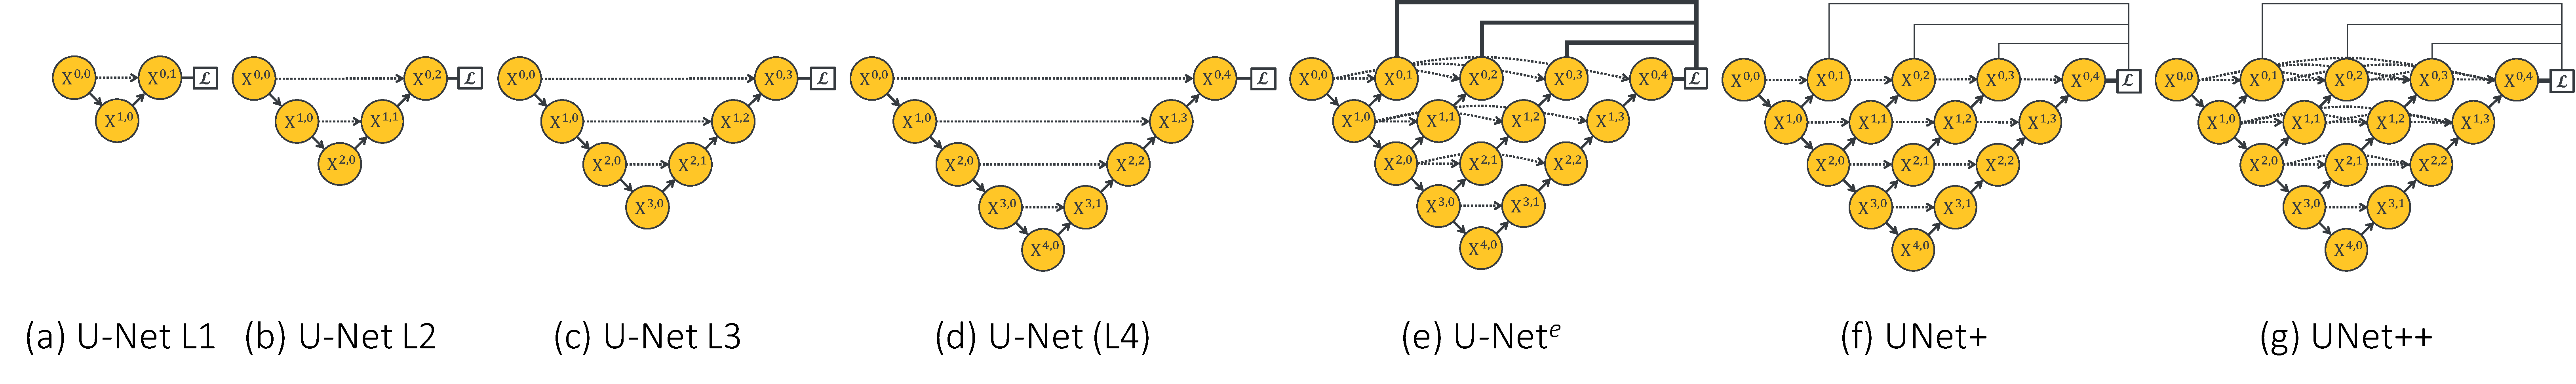
\includegraphics[width=1.0\columnwidth]{Figures/CH4/fig_architecture_evolution.pdf}
\end{center}
\caption[Evolution from U-Net to UNet++]{
Evolution from U-Net to UNet++. Each node in the graph represents a convolution block, downward arrows indicate down-sampling, upward arrows indicate up-sampling, and dot arrows indicate skip connections. (a--d) U-Nets of varying depths. (e) Ensemble architecture, U-Net$^e$, which combines U-Nets of varying depths into one unified architecture. All U-Nets (partially) share the same encoder, but have their own decoders.
(f) UNet+ is constructed from U-Net$^e$ by dropping the original skip connections and connecting every two adjacent nodes with a short skip connection, enabling the deeper decoders to send supervision signals to the shallower decoders. (g) UNet++ is constructed from U-Net$^e$ by connecting the decoders, resulting in densely connected skip connections, enabling dense feature propagation along skip connections and thus more flexible feature fusion at the decoder nodes.
As a result, each node in the UNet++ decoders, from a horizontal perspective, combines multiscale features from its all preceding nodes at the same resolution, and from a vertical perspective, integrates multiscale features across different resolutions from its preceding node, as formulated at Eq.~\ref{eq_unet}. This multiscale feature aggregation of UNet++ gradually synthesizes the segmentation, leading to increased accuracy and faster convergence, as evidenced by our empirical results in~\sectionname~\ref{ch4:experiments}.
Note that, explicit deep supervision is required (bold links) to train U-Net$^e$ but optional (pale links) for UNet+ and UNet++.}
\label{ch4:fig:network_architecture}
\end{sidewaysfigure}

% \fillandplacepagenumber
% \end{landscape}
%##############################################################################################


%##############################################################################################
\begin{table}[t]
\footnotesize
\begin{center}
\begin{threeparttable}
\caption[Ablation Study on U-Nets of Varying Depths]{
Ablation study on U-Nets of varying depths alongside with the new variants of U-Nets proposed in this work. U-Net L$d$ refers to a U-Net with a depth of $d$ (\figurename~\ref{ch4:fig:network_architecture}(a-d)). U-Net$^e$, UNet+, and UNet++ are the new variants of U-Net, which are depicted in \figurename~\ref{ch4:fig:network_architecture}(e-g). ``DS'' denotes deeply supervised training followed by average voting. Intersection over union (IoU) is used as the metric for comparison (mean$\pm$s.d. \%).}
\label{ch4:tab:architecture_analysis}
    \begin{tabular}{p{0.15\linewidth}P{0.04\linewidth}P{0.11\linewidth}P{0.16\linewidth}P{0.16\linewidth}P{0.2\linewidth}}
    \hline
    \textbf{Architecture} & \textbf{DS} & \textbf{Params} & \textbf{EM} & \textbf{Cell} & \textbf{Brain Tumor} \\
    \hline
    U-Net L$1$  & \xmark & 0.1M & 86.83{\tiny $\pm$0.43} & 88.58{\tiny $\pm$1.68} & 86.90{\tiny $\pm$2.25}  \\
    U-Net L$2$  & \xmark & 0.5M & 87.59{\tiny $\pm$0.34} & 89.39{\tiny $\pm$1.64} &  88.71{\tiny $\pm$1.45} \\
    U-Net L$3$   & \xmark & 1.9M & 88.16{\tiny $\pm$0.29} & 90.14{\tiny $\pm$1.57} & 89.62{\tiny $\pm$1.41}  \\
    U-Net (L$4$)  & \xmark & 7.8M & 88.30{\tiny $\pm$0.24} & 88.73{\tiny $\pm$1.64} & 89.21{\tiny $\pm$1.55} \\
    U-Net$^e$  & \cmark  & 8.7M & 88.33{\tiny $\pm$0.23} & 90.72{\tiny $\pm$1.51} &  90.19{\tiny $\pm$0.83} \\
    \hline
    UNet+  & \xmark & 8.7M & 88.39{\tiny $\pm$0.15} & 90.71{\tiny $\pm$1.25} & 90.70{\tiny $\pm$0.91}  \\
    UNet+  & \cmark & 8.7M & 88.89{\tiny $\pm$0.12} & 91.18{\tiny $\pm$1.13} & 91.15{\tiny $\pm$0.65} \\
    \hline
    UNet++  & \xmark & 9.0M & 88.92{\tiny $\pm$0.14} & 91.03{\tiny $\pm$1.34} & 90.86{\tiny $\pm$0.81}\\
    UNet++  & \cmark & 9.0M & \textbf{89.33{\tiny $\pm$0.10}} & \textbf{91.21{\tiny $\pm$0.98}} & {\bf 91.21{\tiny $\pm$0.68}} \\
    \hline
    \end{tabular}
\end{threeparttable}
\end{center}
\end{table}
%##############################################################################################


% \section{Redesigned Skip Connections for Multiscale Feature Aggregation}
\section{Approach \& Property}
\label{ch4:methods}

\figurename~\ref{ch4:fig:network_architecture} shows how UNet++ evolves from the original U-Net. In the following, we first trace this evolution, motivating the need for UNet++, and then explain its technical and implementation details.

\subsection{Evolving Architectural Designs}
\label{ch4:motiv}

We have done a comprehensive ablation study to investigate the performance of U-Nets of varying depths (\figurename~\ref{ch4:fig:network_architecture}(a-d)). For this purpose, we have used three relatively small datasets, namely \texttt{Cell}\footnote{I thank Michael G. Meyer for allowing us to test our ideas on the Cell-CT dataset.}, \texttt{EM}, and \texttt{Brain Tumor} (detailed in~Appendix~\ref{ap1}). \tableautorefname~\ref{ch4:tab:architecture_analysis} summarizes the results. For the cell and brain tumor segmentation, a shallower network (U-Net L$3$)\footnote{In this dissertation, the original notation U-Net/UNet+/UNet++ L$^{d}$ in \citet{zhou2018unet++,zhou2019unet++} has been replaced with U-Net/UNet+/UNet++ L${d}$ to avoid the confusion with footnote symbols.} outperforms the deep U-Net. For the EM dataset, on the other hand, the deeper U-Nets consistently outperform the shallower counterparts, but the  performance gain is only marginal. Our experimental results suggest two key findings: 1) deeper U-Nets are not necessarily always better, 2) the optimal depth of architecture depends on the difficulty and size of the dataset at hand. While these findings may encourage an automated neural architecture search, such an approach is hindered by the limited computational resources~\citep{liu2018progressive,zoph2018learning,liu2019auto,zhang2019customizable,li2019partial}. Alternatively, we propose an ensemble architecture, which combines  U-Nets of varying depths into one unified structure. We refer to this architecture as U-Net$^e$ (\figurename~\ref{ch4:fig:network_architecture}(e)). 
We train U-Net$^e$ by defining a separate loss function for each U-Net in the ensemble, \ie X$^{0,j},~j\in\{1,2,3,4\}$. Our deep supervision scheme differs from the commonly used deep supervision in deep image classification and image segmentation networks; in ~\citep{xie2015holistically,chen2016deep,dou20173d,lee2015deeply} the auxiliary loss functions are added to the nodes along the decoder network, \ie X$^{4-j,j},~j\in\{0,1,2,3,4\}$, whereas we apply them on X$^{0,j},~j\in\{1,2,3,4\}$. At the inference time, the output from each U-Net in the ensemble is averaged.


The ensemble architecture (U-Net$^e$) outlined above benefits from knowledge sharing, because all U-Nets within the ensemble partially share the same encoder even though they have their own  decoders. However, this architecture still suffers from two drawbacks. First, the decoders are disconnected---deeper U-Nets do not offer a supervision signal to the decoders of the shallower U-Nets in the ensemble. Second, the common design of skip connections used in the U-Net$^e$ is unnecessarily restrictive, requiring the network to combine the decoder feature maps with only the same-scale feature maps from the encoder. While striking as a natural design,  there is no guarantee that the same-scale feature maps are the best match for the feature fusion. 

To overcome the above limitations, we remove original skip connections from the U-Net$^e$ and connect every two adjacent nodes in the ensemble, resulting in a new architecture, which we refer to as UNet+ (\figurename~\ref{ch4:fig:network_architecture}(f)). Owing to the new connectivity scheme, UNet+ connects the disjoint decoders, enabling gradient back-propagation from the deeper decoders to the shallower counterparts. UNet+ further relaxes the unnecessarily restrictive behaviour of skip connections by presenting each node in the decoders with the aggregation of all feature maps computed in the shallower stream. While using aggregated feature maps at a decoder node is far less restrictive than having only the same-scale feature map from the encoder,  there is still room for improvement. We further propose to use dense connectivity in UNet+,  resulting in our final architecture proposal, which we refer to as UNet++ (\figurename~\ref{ch4:fig:network_architecture}(g)). With dense connectivity, each node in a decoder is presented with not only the final aggregated feature maps but also with the intermediate aggregated feature maps and the original same-scale feature maps from the encoder. As such, the aggregation layer in the decoder node may learn to use only the same-scale encoder feature maps or use all collected feature maps available at the gate.
Unlike U-Net$^e$, deep supervision is not required for UNet+ and UNet++, however, as we will describe later, deep supervision enables model pruning during the inference time, leading to a significant speedup with only modest drop in  performance.

\subsection{Redesigning Skip Connections}
\label{ch4:model}

Let $x^{i,j}$ denote the output of node X$^{i,j}$ where $i$ indexes the down-sampling layer along the encoder and $j$ indexes the convolution layer of the dense block along the skip connection. The stack of feature maps represented by $x^{i,j}$ is computed as
\begin{equation}
\label{eq_unet}
    x^{i,j}=\begin{cases}
      \mathcal{H}\left(\mathcal{D}(x^{i-1,j})\right),  & j=0  \\
      \mathcal{H}\left(\left[\left[x^{i,k}\right]_{k=0}^{j-1}, \mathcal{U}(x^{i+1,j-1}) \right]\right), & j>0  \\
    \end{cases}
\end{equation}
where function $\mathcal{H}(\cdot)$ is a convolution operation followed by an activation function, $\mathcal{D}(\cdot)$ and $\mathcal{U}(\cdot)$ denote a down-sampling layer and an up-sampling layer respectively, and $[$ $]$ denotes the concatenation layer. Basically, as shown in~\figurename~\ref{ch4:fig:network_architecture}(g), nodes at level $j=0$  receive only one input from the previous layer of the encoder; nodes at level $j=1$ receive two inputs, both from the encoder sub-network but at two consecutive levels; and nodes at level $j>1$ receive $j+1$ inputs, of which $j$ inputs are the outputs of the previous $j$ nodes in the same skip connection and the $j+1^{th}$ input is the up-sampled output from the lower skip connection. The reason that all prior feature maps accumulate and arrive at the current node is because we make use of a dense convolution block along each skip connection.

%##############################################################################################
\begin{figure}[t]
\begin{center}
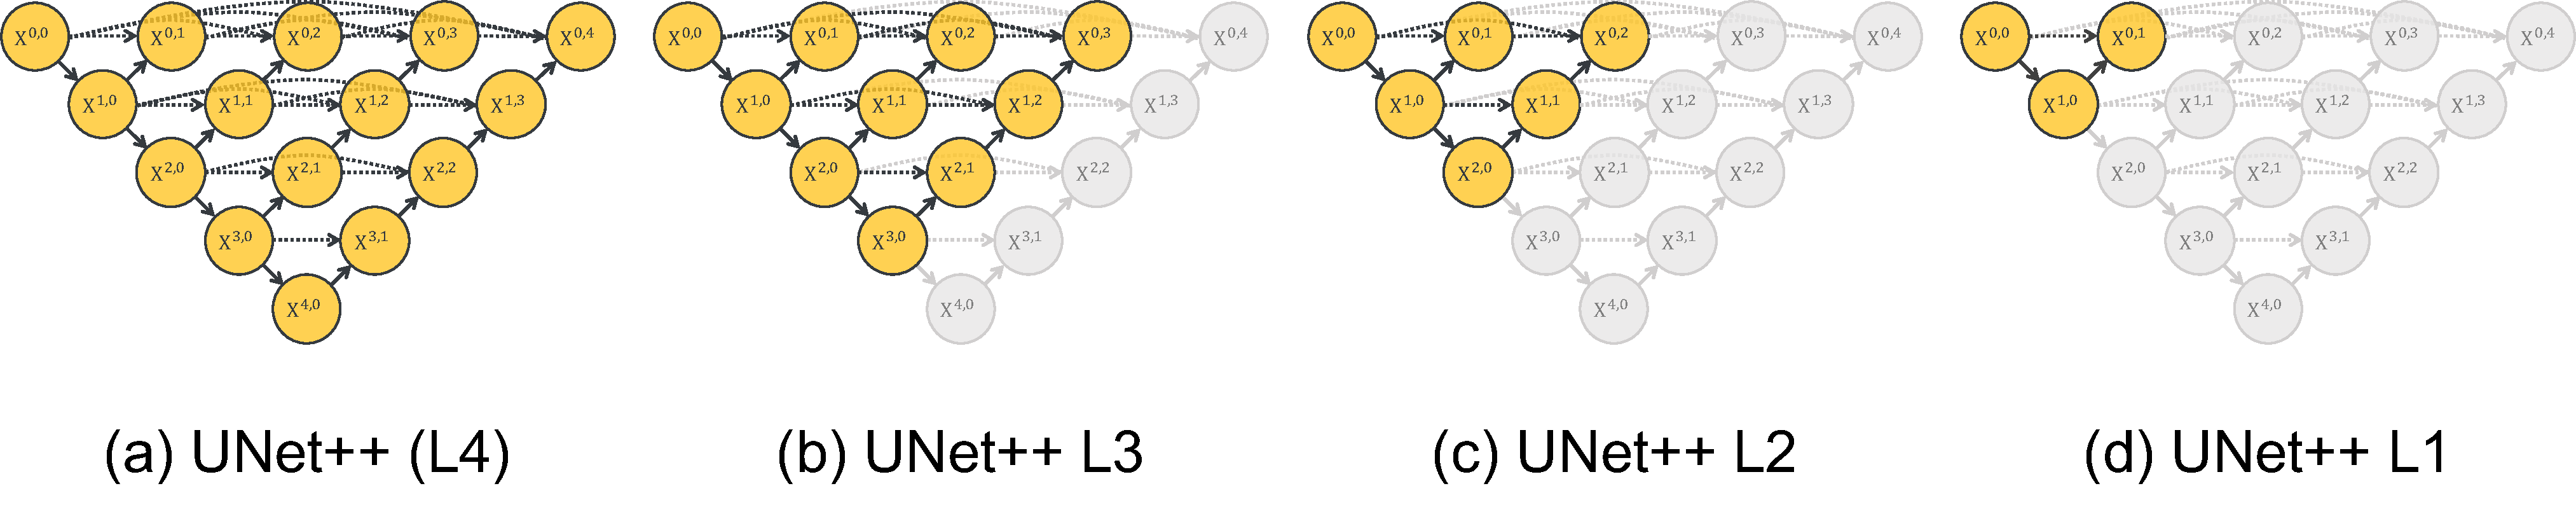
\includegraphics[width=1.0\linewidth]{Figures/CH4/fig_pruned_structure.pdf}
\end{center}
\caption[Deep Supervision Enables Model Pruning]{
Training UNet++ with deep supervision makes segmentation results available at multiple nodes X$^{0,j}$, enabling architecture pruning at inference time. Taking the segmentation result from X$^{0,4}$ leads to no pruning, UNet++ (L$4$),  whereas taking the segmentation result from X$^{0,1}$ results in a maximally pruned architecture, UNet++ L$1$. Note that nodes removed during pruning are colored in gray.}
\label{ch4:fig:prune_structure}
\end{figure}
%##############################################################################################


\subsection{Introducing Deep Supervision}
We introduce deep supervision in UNet++. For this purpose, we append a 1$\times$1 convolution with $\mathcal{C}$ kernels followed by a \textit{Sigmoid} activation function to the outputs from nodes  X$^{0,1}$, X$^{0,2}$, X$^{0,3}$, and X$^{0,4}$ where $\mathcal{C}$ is the number of classes observed in the given dataset. We then define a hybrid segmentation loss consisting of pixel-wise cross-entropy loss and soft dice-coefficient loss for each semantic scale. The hybrid loss may take advantages of what both loss functions have to offer: smooth gradient and handling of class imbalance~\citep{milletari2016v,sudre2017generalised}. Mathematically, the hybrid loss is defined as: 

\begin{equation}
\label{eq:object_function}
\mathcal{L}(Y,P) = -\frac{1}{N}\sum_{c=1}^{\mathcal{C}}\sum_{n=1}^{N}{\left(y_{n,c}\log{p_{n,c}}+\frac{2y_{n,c}p_{n,c}}{y^2_{n,c}+p^2_{n,c}}\right)}
\end{equation}
\noindent where $y_{n,c}\in Y$ and $p_{n,c}\in P$ denote the target labels and predicted probabilities for class $c$ and $n^{th}$ pixel in the batch, $N$ indicates the number of pixels within one batch. The overall loss function for UNet++ is then defined as the weighted summation of the hybrid loss from each individual decoders: $\mathcal{L}=\sum_{i=1}^{d}{\eta_i\cdot \mathcal{L}(Y,P^i)}$, where $d$ indexes the decoder. In the experiments, we give same balanced weights $\eta_i$ to each loss, \ie $\eta_i\equiv 1$, and do not process the ground truth for different outputs supervision like Gaussian blur.

Deep supervision enables model pruning. Owing to deep supervision, UNet++ can be deployed in two operation modes: 1) ensemble mode where the segmentation results from all segmentation branches are collected and then averaged, and 2) pruned mode where the segmentation output is selected from only one of the segmentation branches, the choice of which determines the extent of model pruning and speed gain.  \figurename~\ref{ch4:fig:prune_structure} shows how the choice of the segmentation branch results in pruned architectures of varying complexity. Specifically, taking the segmentation result from X$^{0,4}$ leads to no pruning whereas taking the segmentation result from X$^{0,1}$ leads to maximal pruning of the network.


\subsection{Two Unique Properties}
\label{ch4:approach_property:several_unique_properties}

\begin{enumerate}

    \item \textit{UNet++ enables multi-scale feature aggregation.} The original U-Net carried residual connections between the encoder and decoder, while our UNet++ suggests dense connections in between, reducing semantic gaps and encouraging feature reuse. This idea can be adapted to the original U-Net, the U-Nets with various backbones as feature extractors, and other segmentation frameworks such as Mask RCNN.
    
    \item \textit{UNet++ introduces deep supervision.} Multiple branches in the UNet++ are collaboratively trained with deep supervision at the full resolution. Deep supervision can stabilize the model training and explore the most effective features for varying sizes of lesions. Moreover, deep supervision makes segmentation outputs available at multiple branches, enabling architecture pruning at inference time.
    
    
\end{enumerate}

%##############################################################################################
\begin{table}[t]
\footnotesize
\centering
\caption[Parameter Settings of U-Net, Wide U-Net, UNet+, and UNet++]{
Details of the architectures used in our study. Wider version of U-Net and V-Net are designed to have comparable number of parameters to UNet++ and VNet++.}
\label{ch4:tab:wide_unet} %
\begin{tabular}{P{0.23\linewidth}P{0.12\linewidth}P{0.09\linewidth}P{0.09\linewidth}P{0.09\linewidth}P{0.09\linewidth}P{0.09\linewidth}}
    \hline
    \multirow{2}*{\textbf{Architecture}} & \multirow{2}*{\textbf{Params}} & \textbf{X$^{0,0}$} & \textbf{X$^{1,0}$} & \textbf{X$^{2,0}$} & \textbf{X$^{3,0}$} & \textbf{X$^{4,0}$} \\
     &  & \textbf{X$^{0,4}$} & \textbf{X$^{1,3}$} & \textbf{X$^{2,2}$} & \textbf{X$^{3,1}$} & \textbf{X$^{4,0}$} \\
    \hline
    U-Net & 7.8M &32 & 64 & 128 & 256 & 512 \\
    wide U-Net & 9.1M & 35 & 70 & 140 & 280 & 560 \\
    V-Net & 22.6M & 32 & 64 & 128 & 256 & 512 \\
    wide V-Net & 27.0M & 35 & 70 & 140 & 280 & 560 \\
    \hline
    \textbf{Architecture} & \textbf{Params} & \textbf{X$^{0,0-4}$} & \textbf{X$^{1,0-3}$} & \textbf{X$^{2,0-2}$} & \textbf{X$^{3,0-1}$} & \textbf{X$^{4,0}$} \\
    \hline
    UNet+ & 8.7M &32 & 64 & 128 & 256 & 512 \\
    UNet++ & 9.0M &32 & 64 & 128 & 256 & 512 \\
    VNet+ & 25.3M & 32 & 64 & 128 & 256 & 512 \\
    VNet++ & 26.2M & 32 & 64 & 128 & 256 & 512 \\
    \hline
\end{tabular}
\end{table}
%##############################################################################################


\section{Experiment \& Result}
\label{ch4:experiments}



\subsection{Benchmarking UNet++}
\label{ch4:implementation}

For comparison, we use the original U-Net~\citep{ronneberger2015u} and a customized wide U-Net architecture for 2D segmentation tasks, and V-Net~\citep{milletari2016v} and a customized wide V-Net architecture for 3D segmentation tasks. We choose U-Net (or V-Net for 3D) because it is a common performance baseline for image segmentation. We have also designed a wide U-Net (or wide V-Net for 3D) with a similar number of parameters to our suggested architecture. This is to ensure that the performance gain yielded by our architecture is \textit{not} simply due to the increased number of parameters. \tableautorefname~\ref{ch4:tab:wide_unet} details the U-Net and wide U-Net architectures. We have further compared the performance of UNet++ against UNet+, which is our intermediate architecture proposal. The numbers of kernels in the intermediate nodes have been given in~\tableautorefname~\ref{ch4:tab:wide_unet}. 


%%%%%%%%%%%%%%%%%%%%%%%%%%%%%%%%%%%%%%%%%%%%
% \begin{landscape}
% \thispagestyle{empty}

\begin{sidewaystable}
\begin{threeparttable}[t]
\scriptsize
\begin{center}
    \caption[UNet++ Outperforms U-Net in Semantic Segmentation]{
    Semantic segmentation results measured by IoU (mean$\pm$s.d.) for U-Net, wide U-Net, UNet+ (our intermediate proposal), and  UNet++ (our final proposal). Both UNet+ and UNet++ are evaluated with and without deep supervision (DS). We have performed independent two sample $t$-test between U-Net~\cite{falk2018u} vs. others for 20 independent trials and highlighted boxes in red when the differences are statistically significant ($p<0.05$).}
    \label{ch4:tab:main_results}
    \begin{tabular}{P{0.09\linewidth}P{0.01\linewidth}P{0.05\linewidth}|P{0.07\linewidth}P{0.07\linewidth}P{0.07\linewidth}P{0.07\linewidth}P{0.07\linewidth}|P{0.09\linewidth}P{0.01\linewidth}P{0.05\linewidth}|P{0.11\linewidth}}
    \hline
    \multirow{2}*{\textbf{Architecture}} & \multirow{2}*{\textbf{DS}} & \multirow{2}*{\textbf{Params}} & \multicolumn{5}{c|}{\textbf{2D Application}} & \multirow{2}*{\textbf{Architecture}} & \multirow{2}*{\textbf{DS}} & \multirow{2}*{\textbf{Params}} & \textbf{3D Application} \\
    \cline{4-8}\cline{12-12}
     & & &  \textbf{EM} & \textbf{Cell} & \textbf{Nuclei} & \textbf{BraTS} & \textbf{Liver} & & & & \textbf{Lung Nodule} \\
    \hline
    U-Net & \xmark & 7.8M & 88.30{\tiny $\pm$0.24} & 88.73{\tiny $\pm$1.64} & 90.57{\tiny $\pm$1.26} & 89.21{\tiny $\pm$1.55} & 79.90{\tiny $\pm$1.38} & V-Net & \xmark & 22.6M & 71.17{\tiny $\pm$4.53} \\
    wide U-Net & \xmark & 9.1M & 88.37{\tiny $\pm$0.13} & 88.91{\tiny $\pm$1.43} & 90.47{\tiny $\pm$1.15} & 89.35{\tiny $\pm$1.49}  & 80.25{\tiny $\pm$1.31} & wide V-Net & \xmark & 27.0M & 73.12{\tiny $\pm$3.99} \\
    UNet+ & \xmark & 8.7M & 88.39{\tiny $\pm$0.15} & \cellcolor{maroon!15}90.71{\tiny $\pm$1.25} & \cellcolor{maroon!15}91.73{\tiny $\pm$1.09} & \cellcolor{maroon!15}90.70{\tiny $\pm$0.91} & 79.62{\tiny $\pm$1.20} & VNet+ & \xmark & 25.3M & \cellcolor{maroon!15}75.93{\tiny $\pm$2.93} \\
    UNet+ & \cmark & 8.7M & \cellcolor{maroon!15}88.89{\tiny $\pm$0.12} & \cellcolor{maroon!15}91.18{\tiny $\pm$1.13} & \cellcolor{maroon!15}92.04{\tiny $\pm$0.89} & \cellcolor{maroon!15}91.15{\tiny $\pm$0.65} & \cellcolor{maroon!15}\textbf{82.83{\tiny $\pm$0.92}} & VNet+ & \cmark & 25.3M & \cellcolor{maroon!15}76.72{\tiny $\pm$2.48} \\
    UNet++ & \xmark & 9.0M & \cellcolor{maroon!15}88.92{\tiny $\pm$0.14} & \cellcolor{maroon!15}91.03{\tiny $\pm$1.34} &  \cellcolor{maroon!15}\textbf{92.44{\tiny $\pm$1.20}} & \cellcolor{maroon!15}90.86{\tiny $\pm$0.81}&	\cellcolor{maroon!15}82.51{\tiny $\pm$1.29} & VNet++ & \xmark & 26.2M & \cellcolor{maroon!15}76.24{\tiny $\pm$3.11}\\
    UNet++ & \cmark & 9.0M & \cellcolor{maroon!15}\textbf{89.33{\tiny $\pm$0.10}} & \cellcolor{maroon!15}\textbf{91.21{\tiny $\pm$0.98}}  & \cellcolor{maroon!15}92.37{\tiny $\pm$0.98} & \cellcolor{maroon!15}\textbf{91.21{\tiny $\pm$0.68}}	& \cellcolor{maroon!15}82.60{\tiny $\pm$1.11} & VNet++ & \cmark & 26.2M & \cellcolor{maroon!15}\textbf{77.05{\tiny $\pm$2.42}}\\
    \hline
    \end{tabular}
    \begin{tablenotes}
        \scriptsize
        \item[1] The winner in BraTS-2013 holds a ``complete'' Dice of 92\%  vs. 90.83$\%\pm$2.46\% (our UNet++ with deep supervision).
    \end{tablenotes}
\end{center}
\end{threeparttable}
\end{sidewaystable}
% \fillandplacepagenumber
% \end{landscape}
%%%%%%%%%%%%%%%%%%%%%%%%%%%%%%%%%%%%%%%%%%%%


%##############################################################################################
% \begin{landscape}
% \thispagestyle{empty}

\begin{sidewaysfigure}
\begin{center}
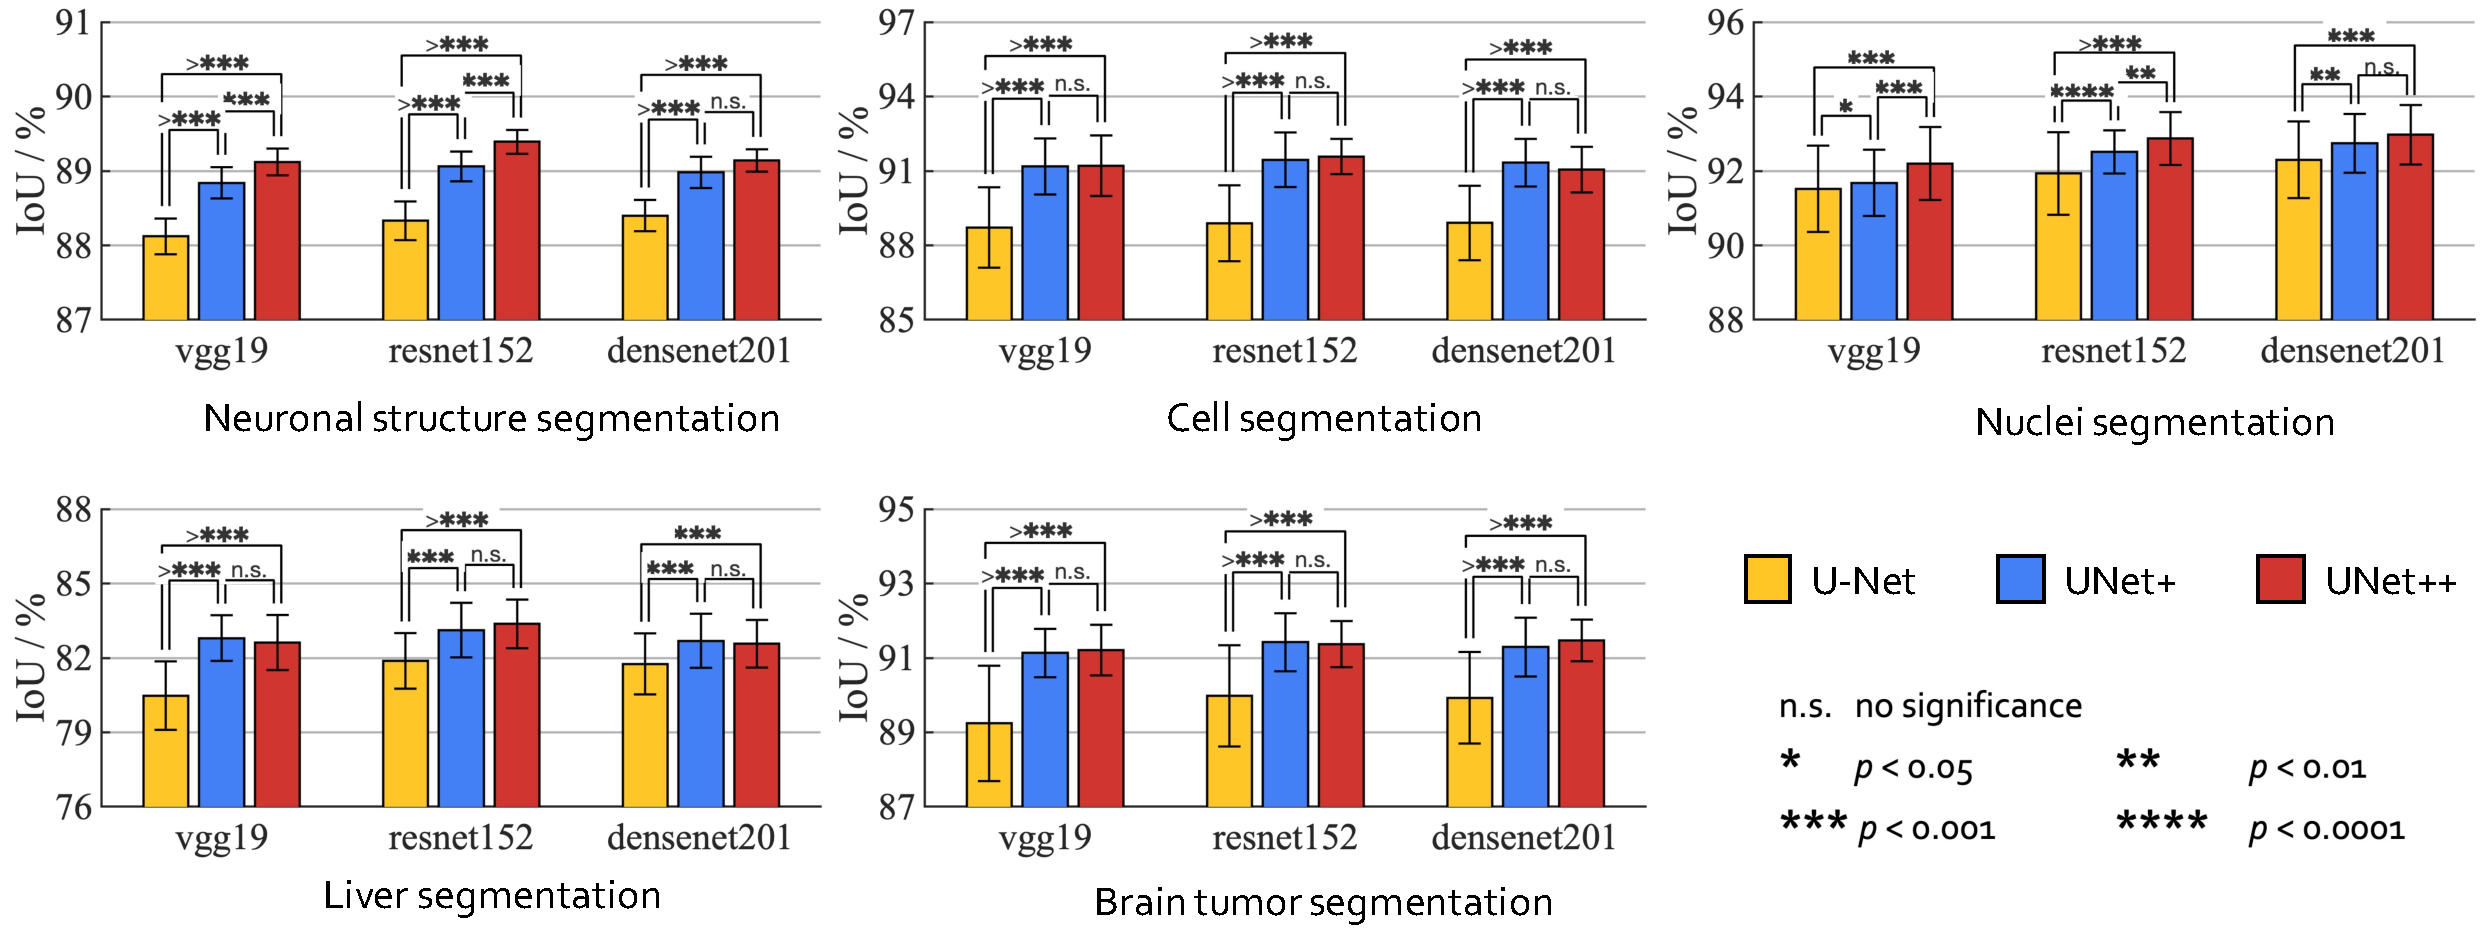
\includegraphics[width=1.0\columnwidth]{Figures/CH4/fig_various_backbones.pdf}
\end{center}
\caption[Comparison of U-Net, UNet+, and UNet++ with Varying Backbones]{
Comparison between U-Net, UNet+, and UNet++ when applied to the state-of-the-art backbones for the tasks of neuronal structure, cell, nuclei, brain tumor, and liver segmentation.
UNet++, trained with deep supervision, consistently outperforms U-Net across all backbone architectures and applications under study. By densely connecting the intermediate layers, UNet++ also yields higher segmentation performance than UNet+ in most experimental configurations.
The error bars represent the 95\% confidence interval and the number of $\ast$ on the bridge indicates the level of significance measured by $p$-value (``n.s.'' stands for ``not statistically significant'').}
\label{ch4:fig:various_backbones}
\end{sidewaysfigure}

% \fillandplacepagenumber
% \end{landscape}
%##############################################################################################


\subsection{UNet++ Outperforms U-Net in Semantic Segmentation}
\label{ch4:semantic_results}

\tableautorefname~\ref{ch4:tab:main_results} compares U-Net, wide U-Net, UNet+, and UNet++ in terms of the number parameters and segmentation results measured by IoU (mean$\pm$s.d) for the six segmentation tasks under study. As seen, wide U-Net consistently outperforms U-Net. This improvement is attributed to the larger number of parameters in wide U-Net. UNet++ without deep supervision achieves a significant IoU gain over both U-Net and wide U-Net for all the six tasks of neuronal structure ($\uparrow$0.62$\pm$0.10, $\uparrow$0.55$\pm$0.01), cell ($\uparrow$2.30$\pm$0.30, $\uparrow$2.12$\pm$0.09), nuclei ($\uparrow$1.87$\pm$0.06, $\uparrow$1.71$\pm$0.06), brain tumor ($\uparrow$2.00$\pm$0.87, $\uparrow$1.86$\pm$0.81), liver\footnote{I acknowledge Md Mahfuzur Rahman Siddiquee, with whom I co-authored~\citet{zhou2018unet++,zhou2019unet++}, for conducting the experiments and providing the results for liver segmentation.} ($\uparrow$2.62$\pm$0.09, $\uparrow$2.26$\pm$0.02), and lung nodule ($\uparrow$5.06$\pm$1.42, $\uparrow$3.12$\pm$0.88) segmentation. Using deep supervision and average voting further improves UNet++, increasing the IoU by up to 0.8 points. Specifically, neuronal structure and lung nodule segmentation benefit the most from deep supervision because they appear at varying scales in EM and CT slices.
Deep supervision, however, is only marginally effective for other datasets at best.  \figurename~\ref{ch4:fig:predict_visualization} depicts a qualitative comparison between the results of U-Net, wide U-Net, and UNet++. 

We have further investigated the extensibility of UNet++ for semantic segmentation by applying redesigned skip connections to an array of modern CNN architectures: vgg-19~\citep{simonyan2014very}, resnet-152~\citep{he2016deep}, and densenet-201~\citep{huang2017densely}. Specifically, we have turned each architecture above into a U-Net model by adding a decoder sub-network, and then replaced the plain skip connections of U-Net with the redesigned connections of UNet++. For comparison, we have also trained U-Net and  UNet+ with the aforementioned backbone architectures. 
For a comprehensive comparison, we have used \texttt{EM}, \texttt{Cell}, \texttt{Nuclei}, \texttt{Brain Tumor} and \texttt{Liver} segmentation datasets.
As seen in \figurename~\ref{ch4:fig:various_backbones}, UNet++ consistently outperforms U-Net and UNet+ across all backbone architectures and applications under study.
Through 20 trials, we further present a statistical analysis based on the independent two-sample $t$-test on each pair among U-Net, UNet+, and UNet++.
Our results suggest that UNet++ is an effective, backbone-agnostic extension to U-Net. 


%##############################################################################################
\begin{figure}[t]
\begin{center}
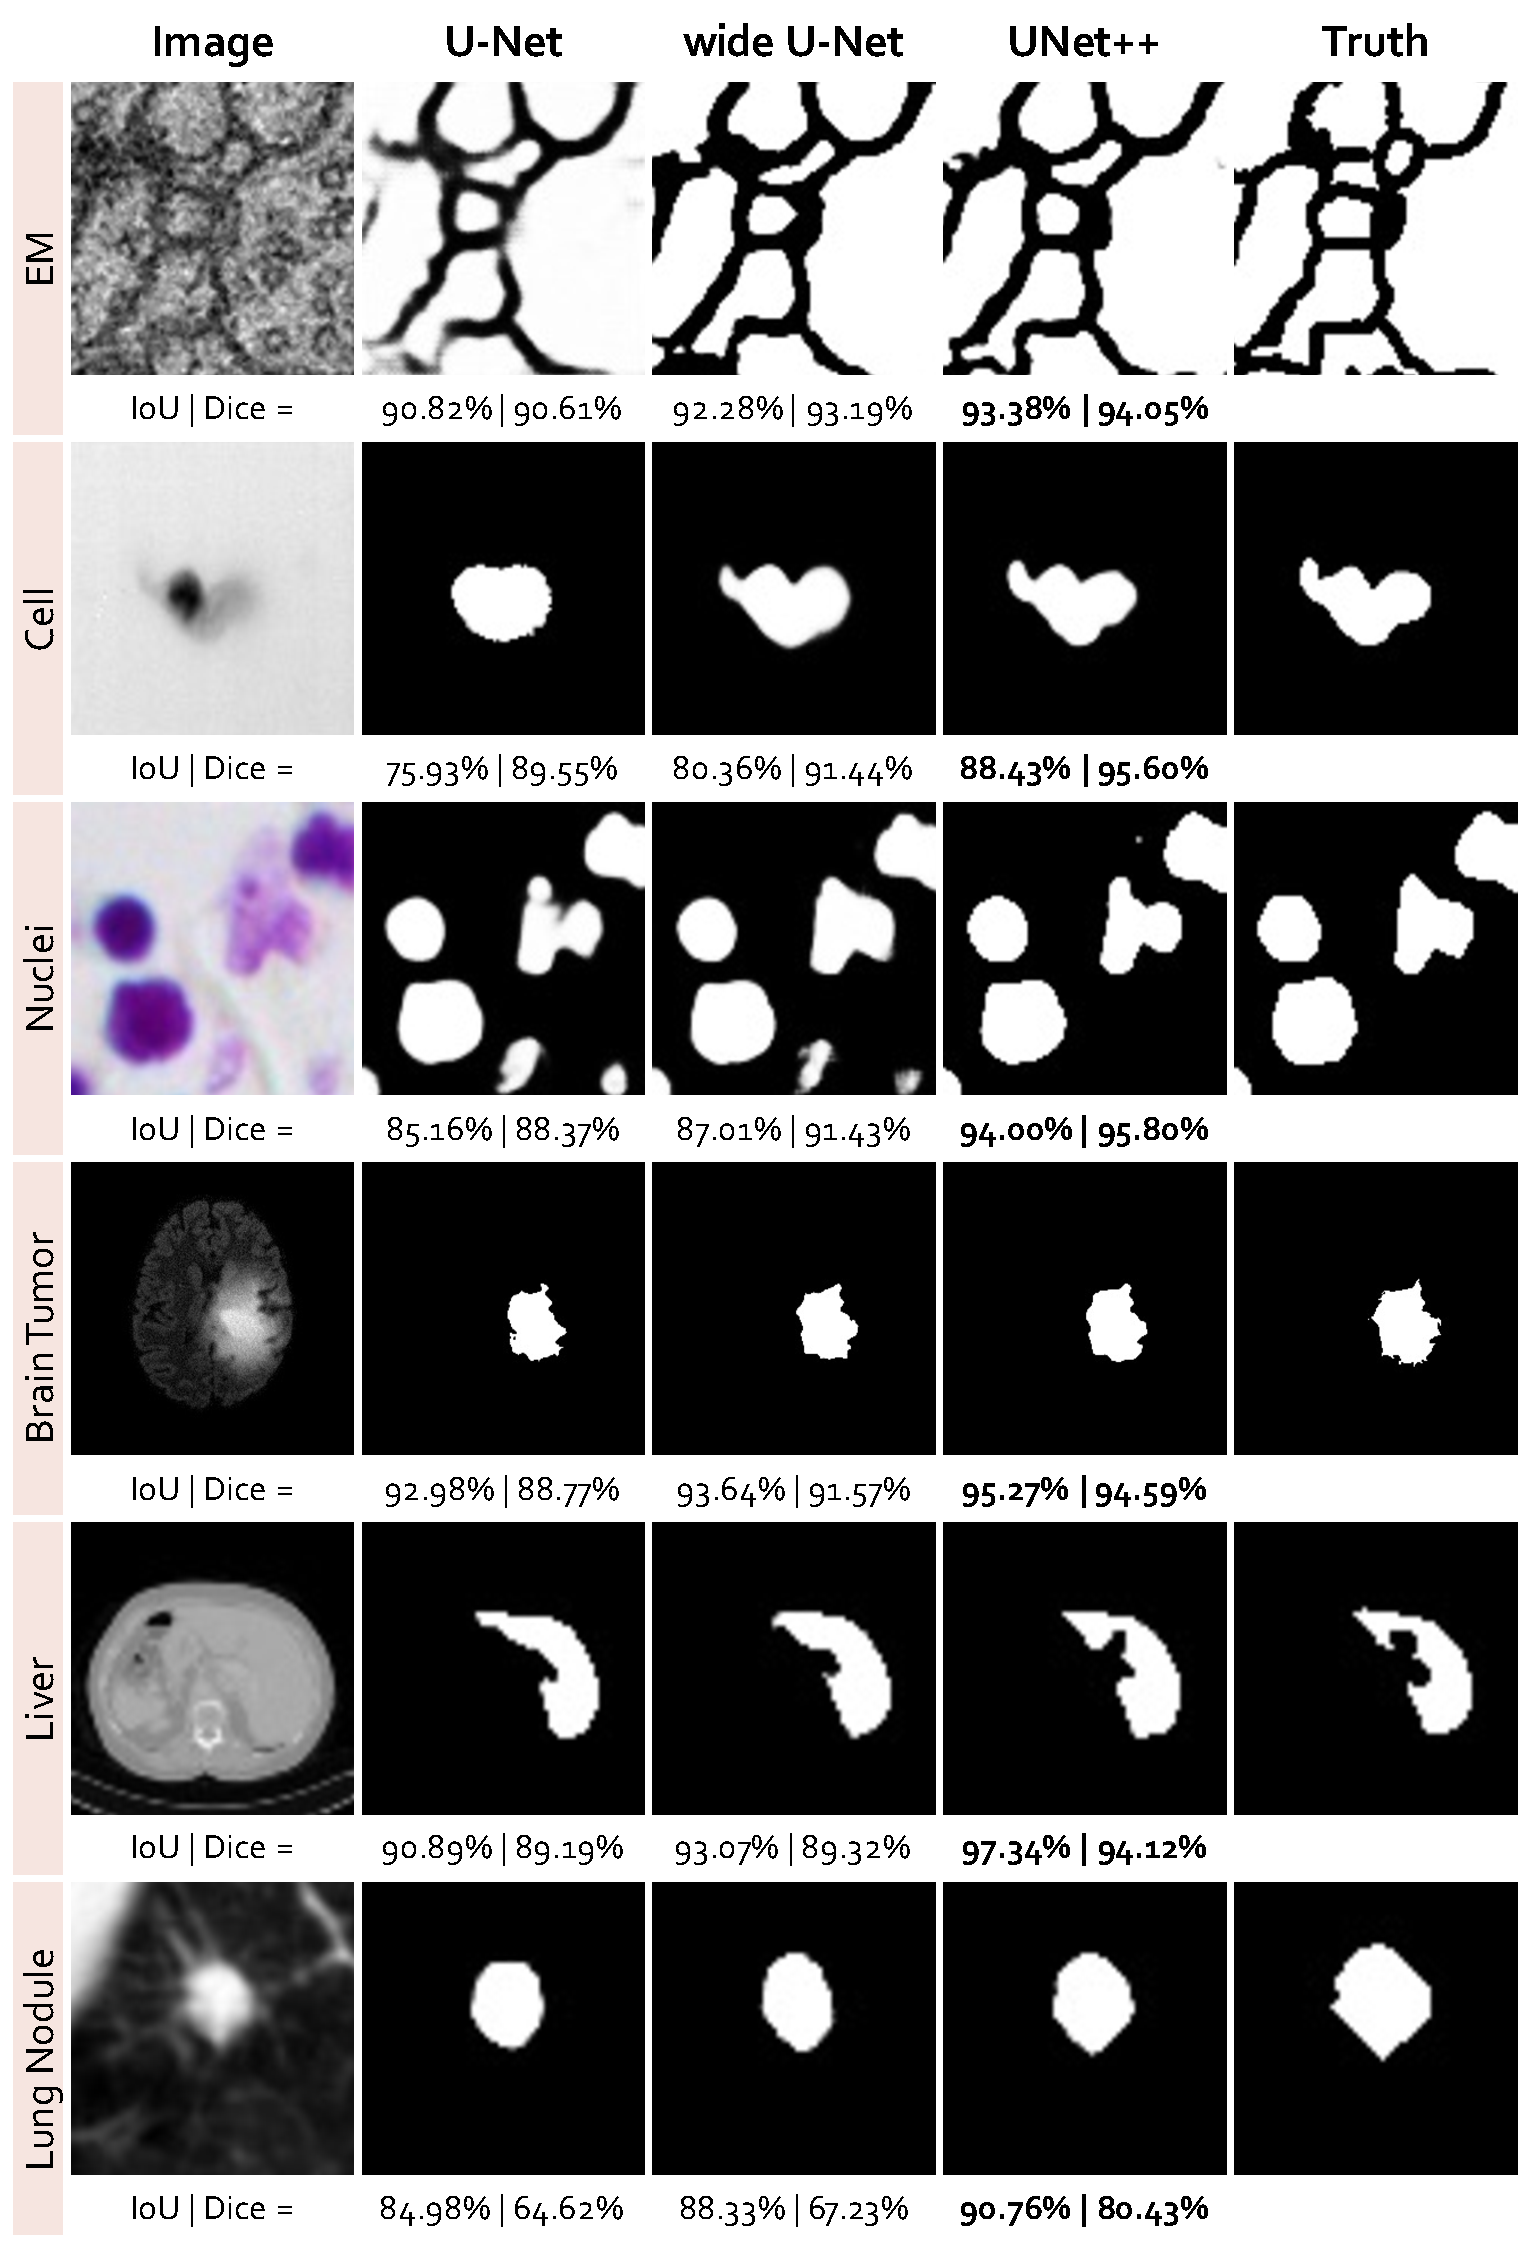
\includegraphics[width=0.6\linewidth]{Figures/CH4/fig_qualitative_comparison.pdf}
\end{center}
\caption[Qualitative Comparison among U-Net, Wide U-Net, and UNet++]{
Qualitative comparison among U-Net, wide U-Net, and UNet++; showing segmentation results for our six distinct biomedical image segmentation applications. They include various 2D and 3D modalities. The corresponding quantitative scores are provided at the bottom of each prediction (IoU $|$ Dice).}
\label{ch4:fig:predict_visualization}
\end{figure}
%##############################################################################################


%##############################################################################################
\begin{table}[t]
\footnotesize
\begin{center}
\begin{threeparttable}
    \caption[Mask RCNN++ Surpasses Mask R-CNN in Instance Segmentation]{
    Redesigned skip connections improve both semantic and instance segmentation for the task of nuclei segmentation. We use Mask R-CNN for instance segmentation and U-Net for semantic segmentation in this comparison.}
    \label{ch4:tab:fcn_family_performance}
    \begin{tabular}{P{0.32\linewidth}P{0.18\linewidth}P{0.12\linewidth}P{0.12\linewidth}P{0.12\linewidth}}
    \hline
     \textbf{Architecture} & \textbf{Backbone} & \textbf{IoU} & \textbf{Dice} & \textbf{Score} \\
    \hline
    U-Net &resnet101&91.03 & 75.73 & 0.244 \\
    \rowcolor{maroon!15}
     UNet++&resnet101&   \bd{92.55} & \bd{89.74} & \bd{0.327} \\
    \hline
    Mask-RCNN &resnet101& 93.28 & 87.91 & 0.401 \\
    \rowcolor{maroon!15}
    MaskRCNN++ &resnet101&\bd{95.10} & \bd{91.36} & \bd{0.414} \\
    \hline
    \end{tabular}
    \begin{tablenotes}
        \scriptsize
        \item[1] Mask R-CNN with UNet++ design in its feature pyramid.
    \end{tablenotes}
\end{threeparttable}
\end{center}
\end{table}
%##############################################################################################


\subsection{MaskRCNN++ Tops Mask-RCNN in Instance Segmentation}
\label{ch4:instance_segmentation}

Instance segmentation consists in segmenting and distinguishing all object instances; hence, more challenging than semantic segmentation. We use Mask R-CNN~\citep{he2017mask} as the baseline model for instance segmentation. Mask R-CNN utilizes feature pyramid network (FPN) as backbone to generate object proposal at multiple scales, and then outputs the segmentation masks for the collected proposals via a dedicated segmentation branch. We modify Mask R-CNN by replacing the plain skip connections of FPN with the redesigned skip connections of UNet++. We refer to this model as Mask RCNN++. We use resnet101 as the backbone for Mask R-CNN in our experiments. 

\tableautorefname~\ref{ch4:tab:fcn_family_performance} compares the performance of Mask R-CNN and Mask RCNN++ for nuclei segmentation.
We have chosen the \texttt{Nuclei} dataset because multiple nucleolus instances can be present in an image, in which case each instance is annotated in a different color, and thus marked as a distinct object. Therefore, this dataset is amenable to both semantic segmentation where all nuclei instances are treated as foreground class, and also instance segmentation where each individual nucleus is to be segmented separately.
As seen in \tableautorefname~\ref{ch4:tab:fcn_family_performance}, Mask RCNN++ outperforms its original counterpart, achieving 1.82 points increase in IoU (93.28\% to 95.10\%), 3.45 points increase in Dice (87.91\% to 91.36\%), and 0.013 points increase in the leaderboard score (0.401 to 0.414). To put this performance in perspective, we have also trained a U-Net and UNet++ model for semantic segmentation with a resnet101 backbone. As seen in \tableautorefname~\ref{ch4:tab:fcn_family_performance}, Mask R-CNN models achieve higher segmentation performance than semantic segmentation models. Furthermore, as expected, UNet++ outperforms U-Net for semantic segmentation.

%##############################################################################################
\begin{figure}[t]
\begin{center}
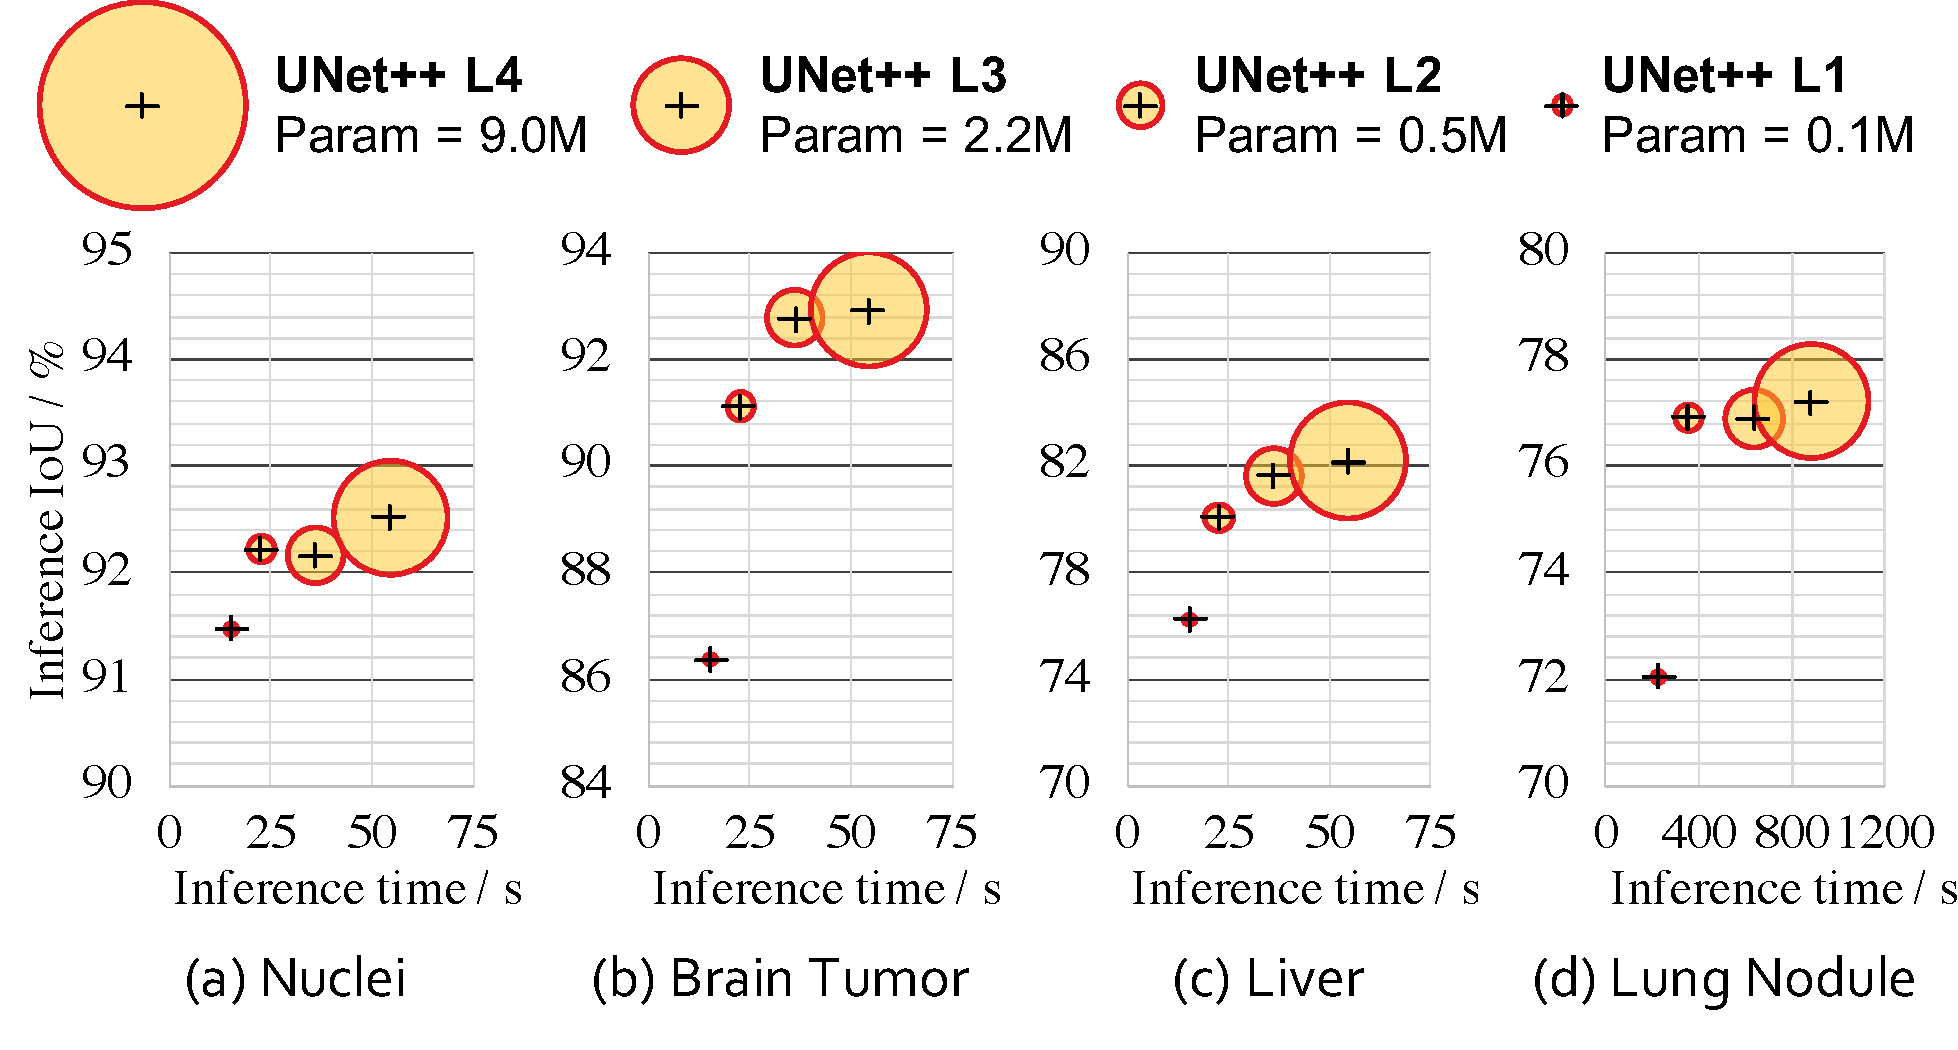
\includegraphics[width=0.8\linewidth]{Figures/CH4/fig_inference_time.pdf}
\end{center}
\caption[UNet++ Accelerates Inference Speed by Model Pruning]{
Complexity (size $\propto$ parameters), inference time, and IoU of UNet++ under different levels of pruning. The inference time is calculated by the time taken to process 10K test images on a single NVIDIA TITAN X (Pascal) GPU with 12 GB memory.}
\label{ch4:fig:speed_accuracy}
\end{figure}
%##############################################################################################



\subsection{UNet++ Accelerates Inference Speed by Model Pruning}
\label{ch4:model_pruning}

Once UNet++ is trained, the decoder path for depth $d$ at inference time is completely independent from the decoder path for depth $d+1$. As a result, we can completely remove the decoder for depth $d+1$, obtaining a shallower version of the trained UNet++ at depth $d$, owing to the introduced deep supervision. This pruning can significantly reduce the inference time, but segmentation performance may degrade. As such, the level of pruning should be determined by evaluating the model's performance on the validation set. We have studied the inference speed-IoU trade-off for UNet++ in \figurename~\ref{ch4:fig:speed_accuracy}. We use UNet++ L$d$ to denote UNet++ pruned at depth $d$ (see \figurename~\ref{ch4:fig:prune_structure} for further details). As seen, UNet++ L${3}$ achieves on average 32.2\% reduction in inference time and 75.6\% reduction in memory footprint while degrading IoU by only 0.6 points. More aggressive pruning further reduces the inference time but at the cost of significant IoU degradation. More importantly, this observation has the potential to exert important impact on computer-aided diagnosis (CAD) on mobile devices, as the existing deep convolutional neural network models are computationally expensive and memory intensive.

%##############################################################################################
\begin{figure}[t]
\begin{center}
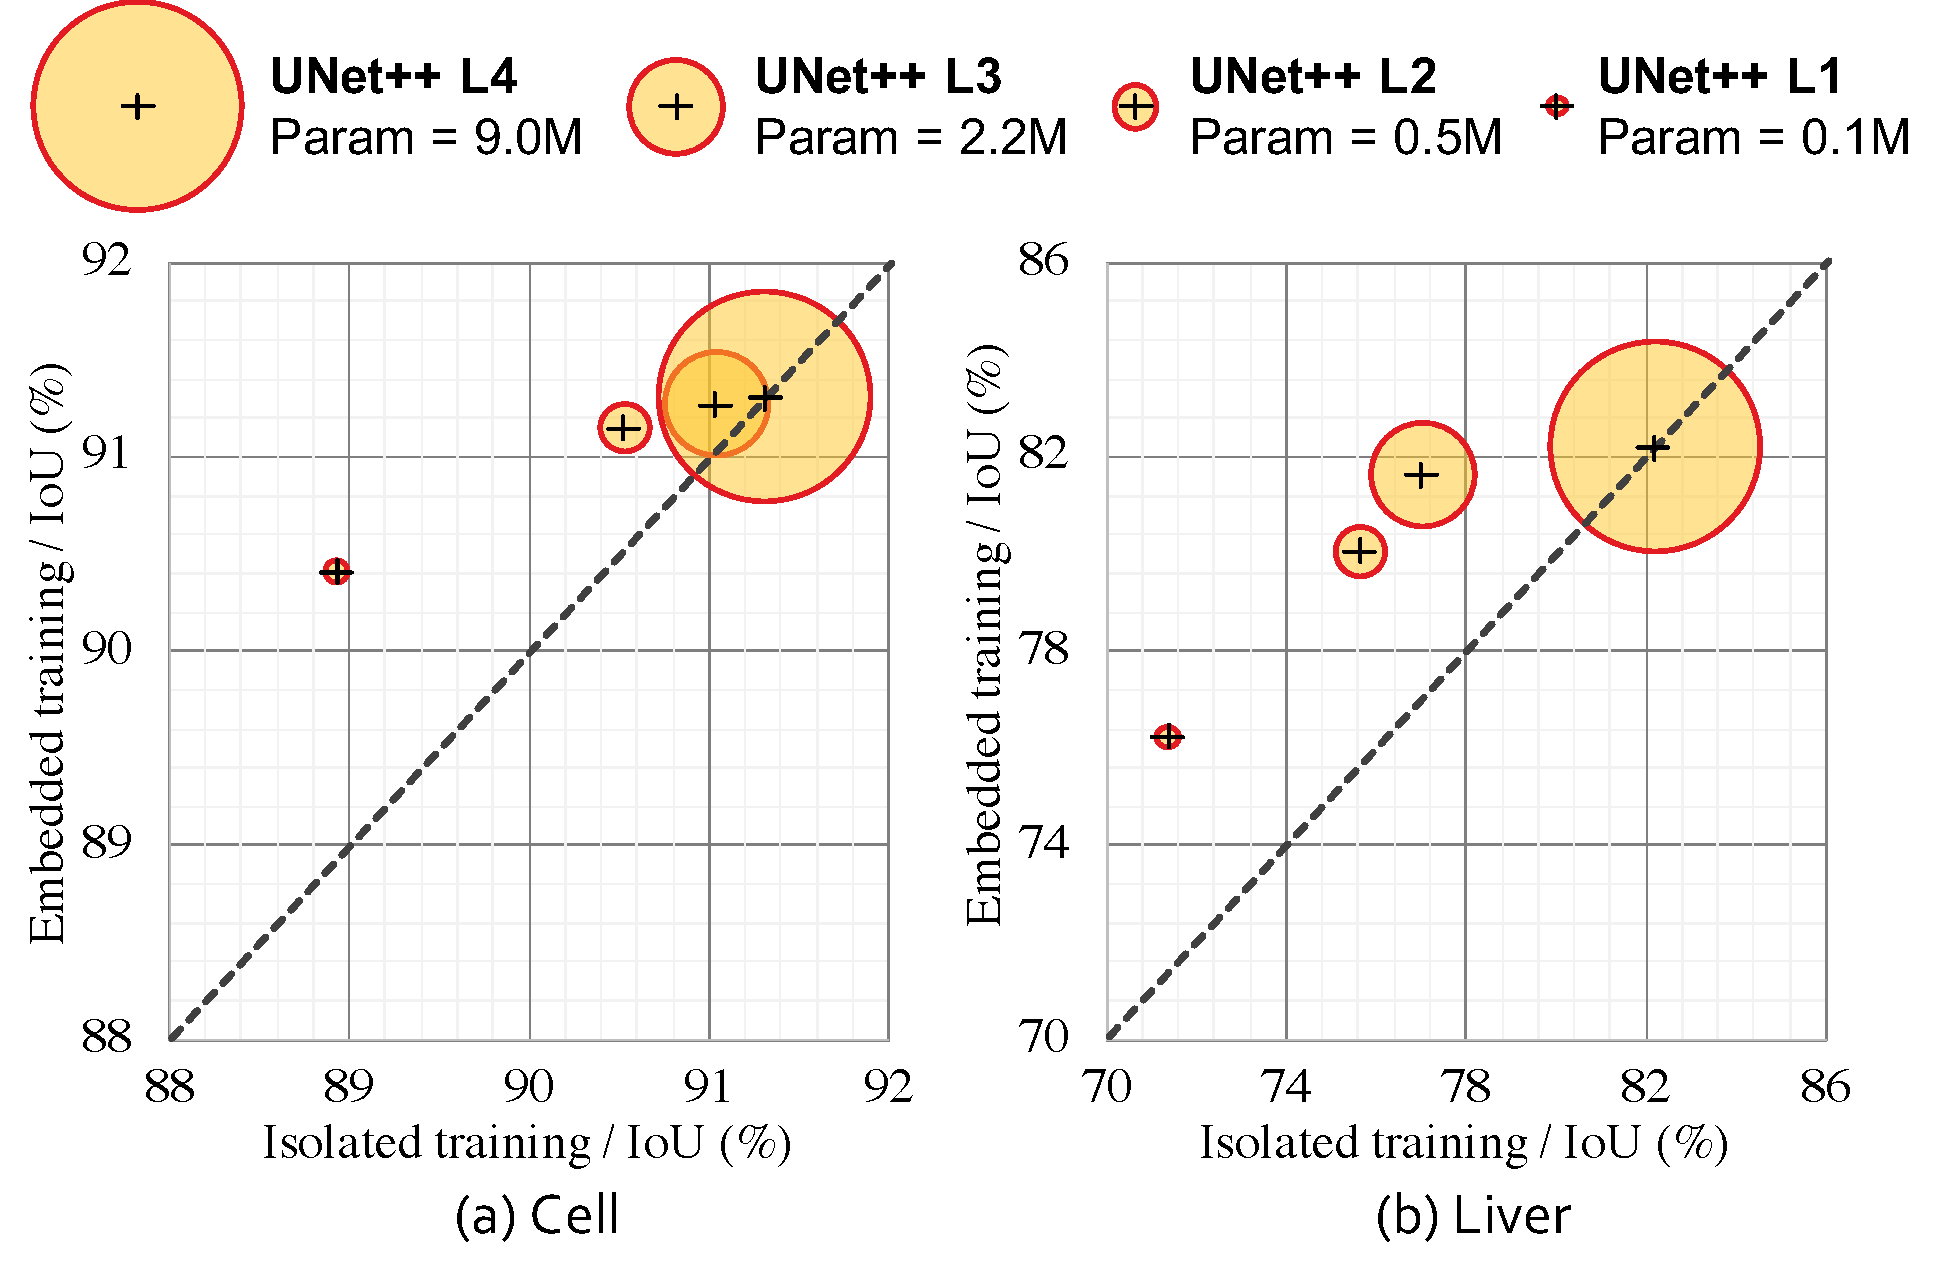
\includegraphics[width=0.8\linewidth]{Figures/CH4/fig_isolated_embedded.pdf}
\end{center}
\caption[Embedded UNet++ Surpasses Isolated U-Nets]{
We demonstrate that our architectural design improves the performance of each shallower network embedded in UNet++. The embedded shallower networks show improved segmentation when pruned from UNet++ in comparison to the same network trained isolated. Due to no pruning, UNet++ L$4$ naturally achieves the same level of performance in isolated and embedded training modes.}
\label{ch4:fig:pruned_vs_stand-alone}
\end{figure}
%##############################################################################################



\subsection{Embedded UNet++ Surpasses Isolated U-Nets}
\label{ch4:embedded_vs_isolated_training}

In theory, UNet++ L$d$ can be trained in two fashions: 1) embedded training where the full UNet++ model is trained and then pruned at depth $d$ to obtain UNet++ L$d$, 2) isolated training where UNet++ L$d$ is trained in isolation without any interactions with the deeper encoder and decoder nodes. Referring to~\figurename~\ref{ch4:fig:prune_structure}, embedded training of a sub-network consists of training all graph nodes (both yellow and grey components) with deep supervision, but we then use only the yellow sub-network during the inference time. In contrast, isolated training consists of removing the grey nodes from the graph, basing the training and test solely on the yellow sub-network.

We have compared the isolated and embedded training schemes for various levels of UNet++ pruning across two datasets in~\figurename~\ref{ch4:fig:pruned_vs_stand-alone}\footnote{I thank Mohammad Reza Hosseinzadeh Taher and Fatemeh Haghighi for their verification of liver segmentation performance and the ablation study of embedded and isolated UNet++.}. We have discovered that the embedded training of UNet++ L$d$ results in a higher performing model than training the same architecture in isolation. The observed superiority is more pronounced under aggressive pruning when the full UNet++ is pruned to UNet++ L$1$. In particular, the embedded training of UNet++ L$1$ for liver segmentation achieves 5-point increase in IoU over the isolated training scheme. This finding suggests that supervision signal coming from the deep downstream enables training higher performing shallower models. This finding is also related to knowledge distillation where the knowledge learned by a deep teacher network is learned by a shallower student network.

%##############################################################################################
\begin{figure}[t]
\begin{center}
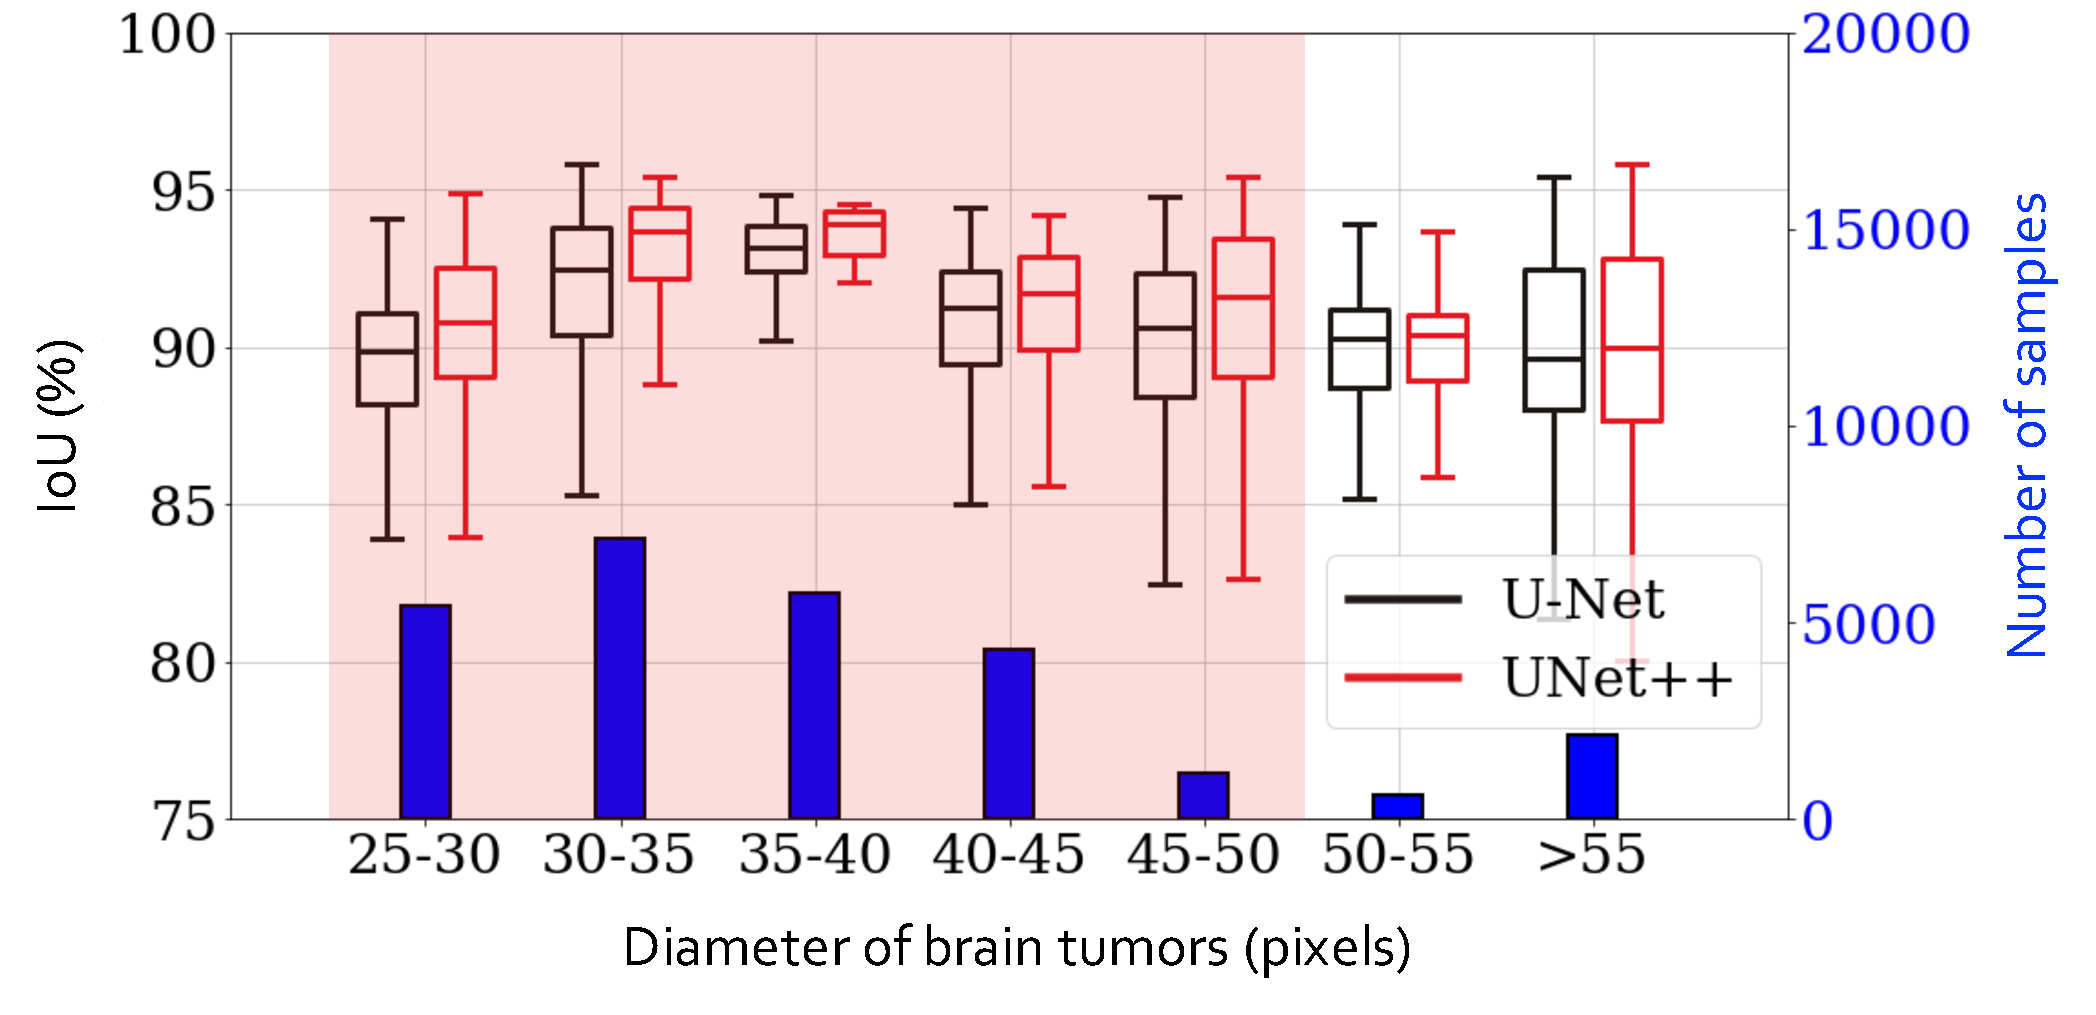
\includegraphics[width=0.85\linewidth]{Figures/CH4/fig_physical_real_brain_tumor_size_stat.pdf}
\end{center}
\caption[UNet++ Can Segment Lesions with Varying Sizes]{
UNet++ can better segment tumors of various sizes than does U-Net. We measure the size of tumors based on the ground truth masks and then divide them into seven groups. The histogram shows the distribution of different tumor sizes. The box-plot compares the segmentation performances of U-Net (black) and UNet++ (red) in each group. The $t$-test for two independent samples has been further performed on each group. As seen, UNet++ improves segmentation for all sizes of tumors and the improvement is significant ($p<0.05$) for the majority of the tumor sizes (highlighted in red).}
\label{ch4:fig:multi_depth_improvement_brain_tumor}
\end{figure}
%##############################################################################################


\section{Discussion \& Conclusion}
\label{ch4:discussion_conclusion}


\subsection{Can UNet++ Segment Lesions with Varying Sizes?}
\label{ch4:discussion_conclusion:stratified_lesion_sizes}

\figurename~\ref{ch4:fig:multi_depth_improvement_brain_tumor} compares U-Net and UNet++ for segmenting different sizes of brain tumors. To avoid clutter in the figure, we group the tumors by size into seven buckets. As seen, UNet++ consistently outperforms U-Net across all the buckets. We also adopt $t$-test on each bucket based on 20 different trials to measure the significance of the improvement, concluding that 5 out of the 7 comparisons are statistically significant ($p < 0.05$). The capability of UNet++ in segmenting tumors of varying sizes is attributed to its built-in ensemble of U-Nets, which enables image segmentation based on multi-receptive field networks.

%##############################################################################################
% \begin{landscape}
% \thispagestyle{empty}

\begin{sidewaysfigure}
\begin{center}
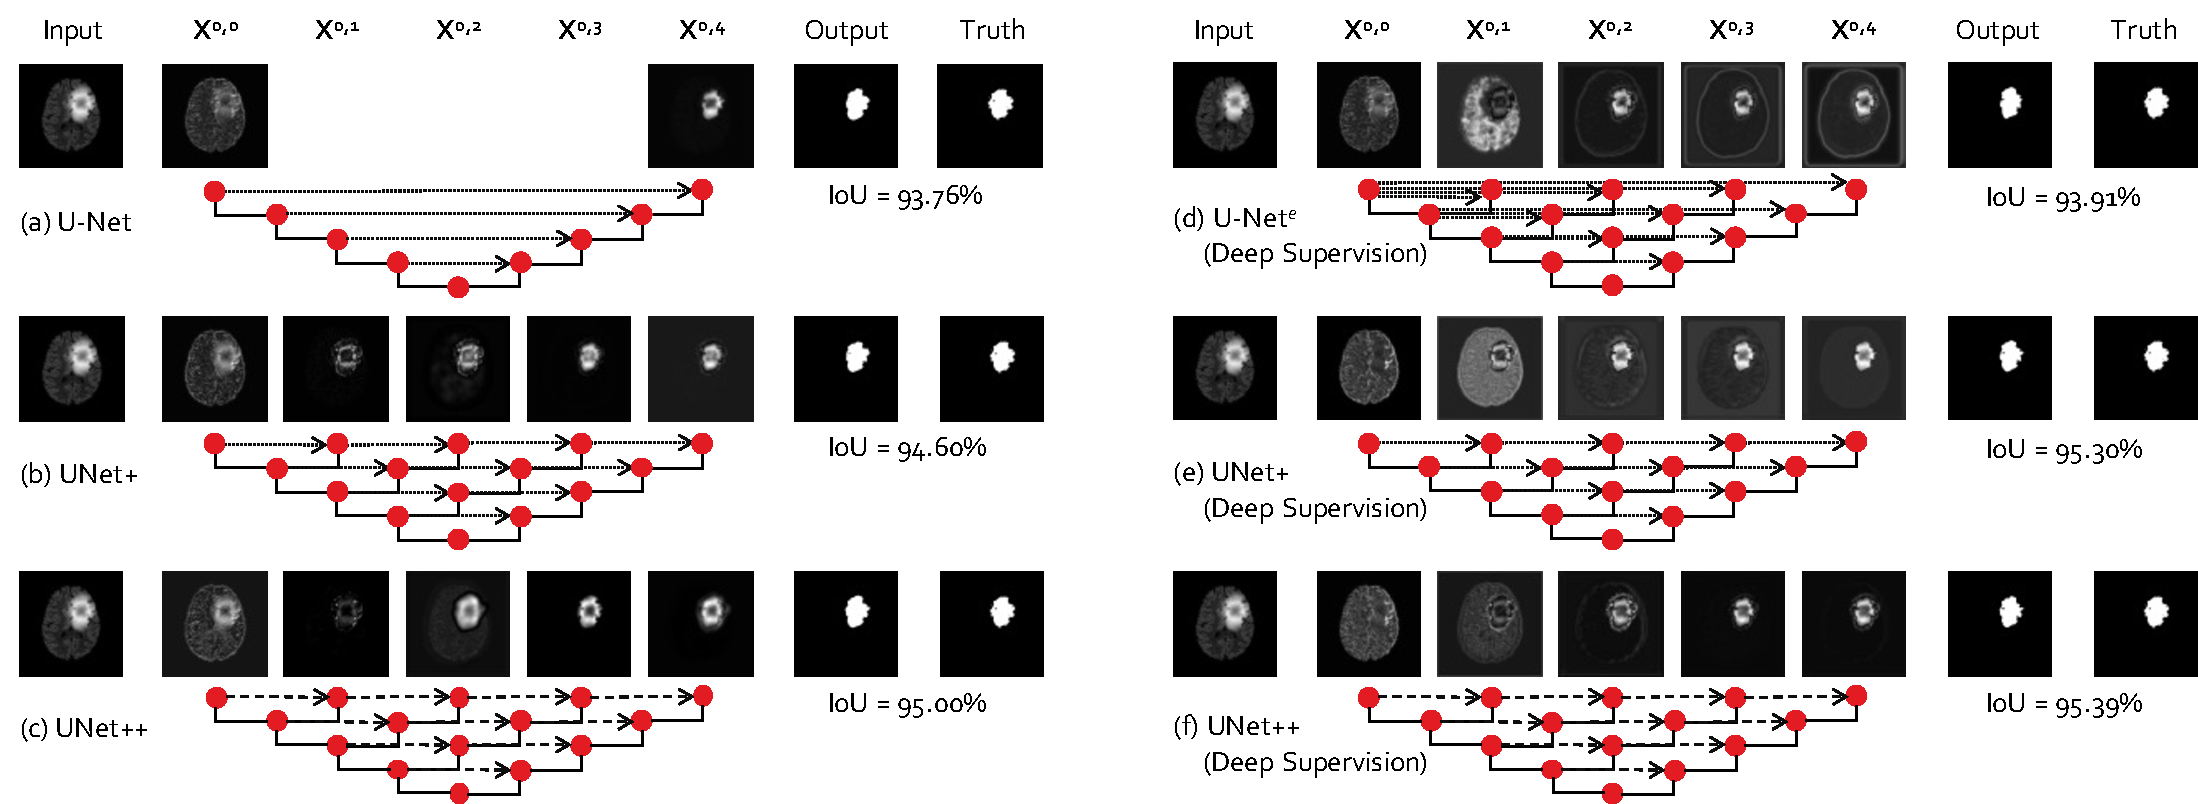
\includegraphics[width=1.0\columnwidth]{Figures/CH4/fig_feature_map_aggregation_brats.pdf}
\end{center}
\caption[Visualization of Multi-scale Feature Map Aggregation]{Visualization and comparison of feature maps from early, intermediate, and late layers along the top most skip connection for brain tumor images. Here, the dot arrows denote the plain skip connection in U-Net and UNet+, while the dash arrows denote dense connections introduced in UNet++.}
\label{ch4:fig:feature_map_aggregation}
\end{sidewaysfigure}

% \fillandplacepagenumber
% \end{landscape}
%##############################################################################################


%##############################################################################################
\begin{figure}[t]
\begin{center}
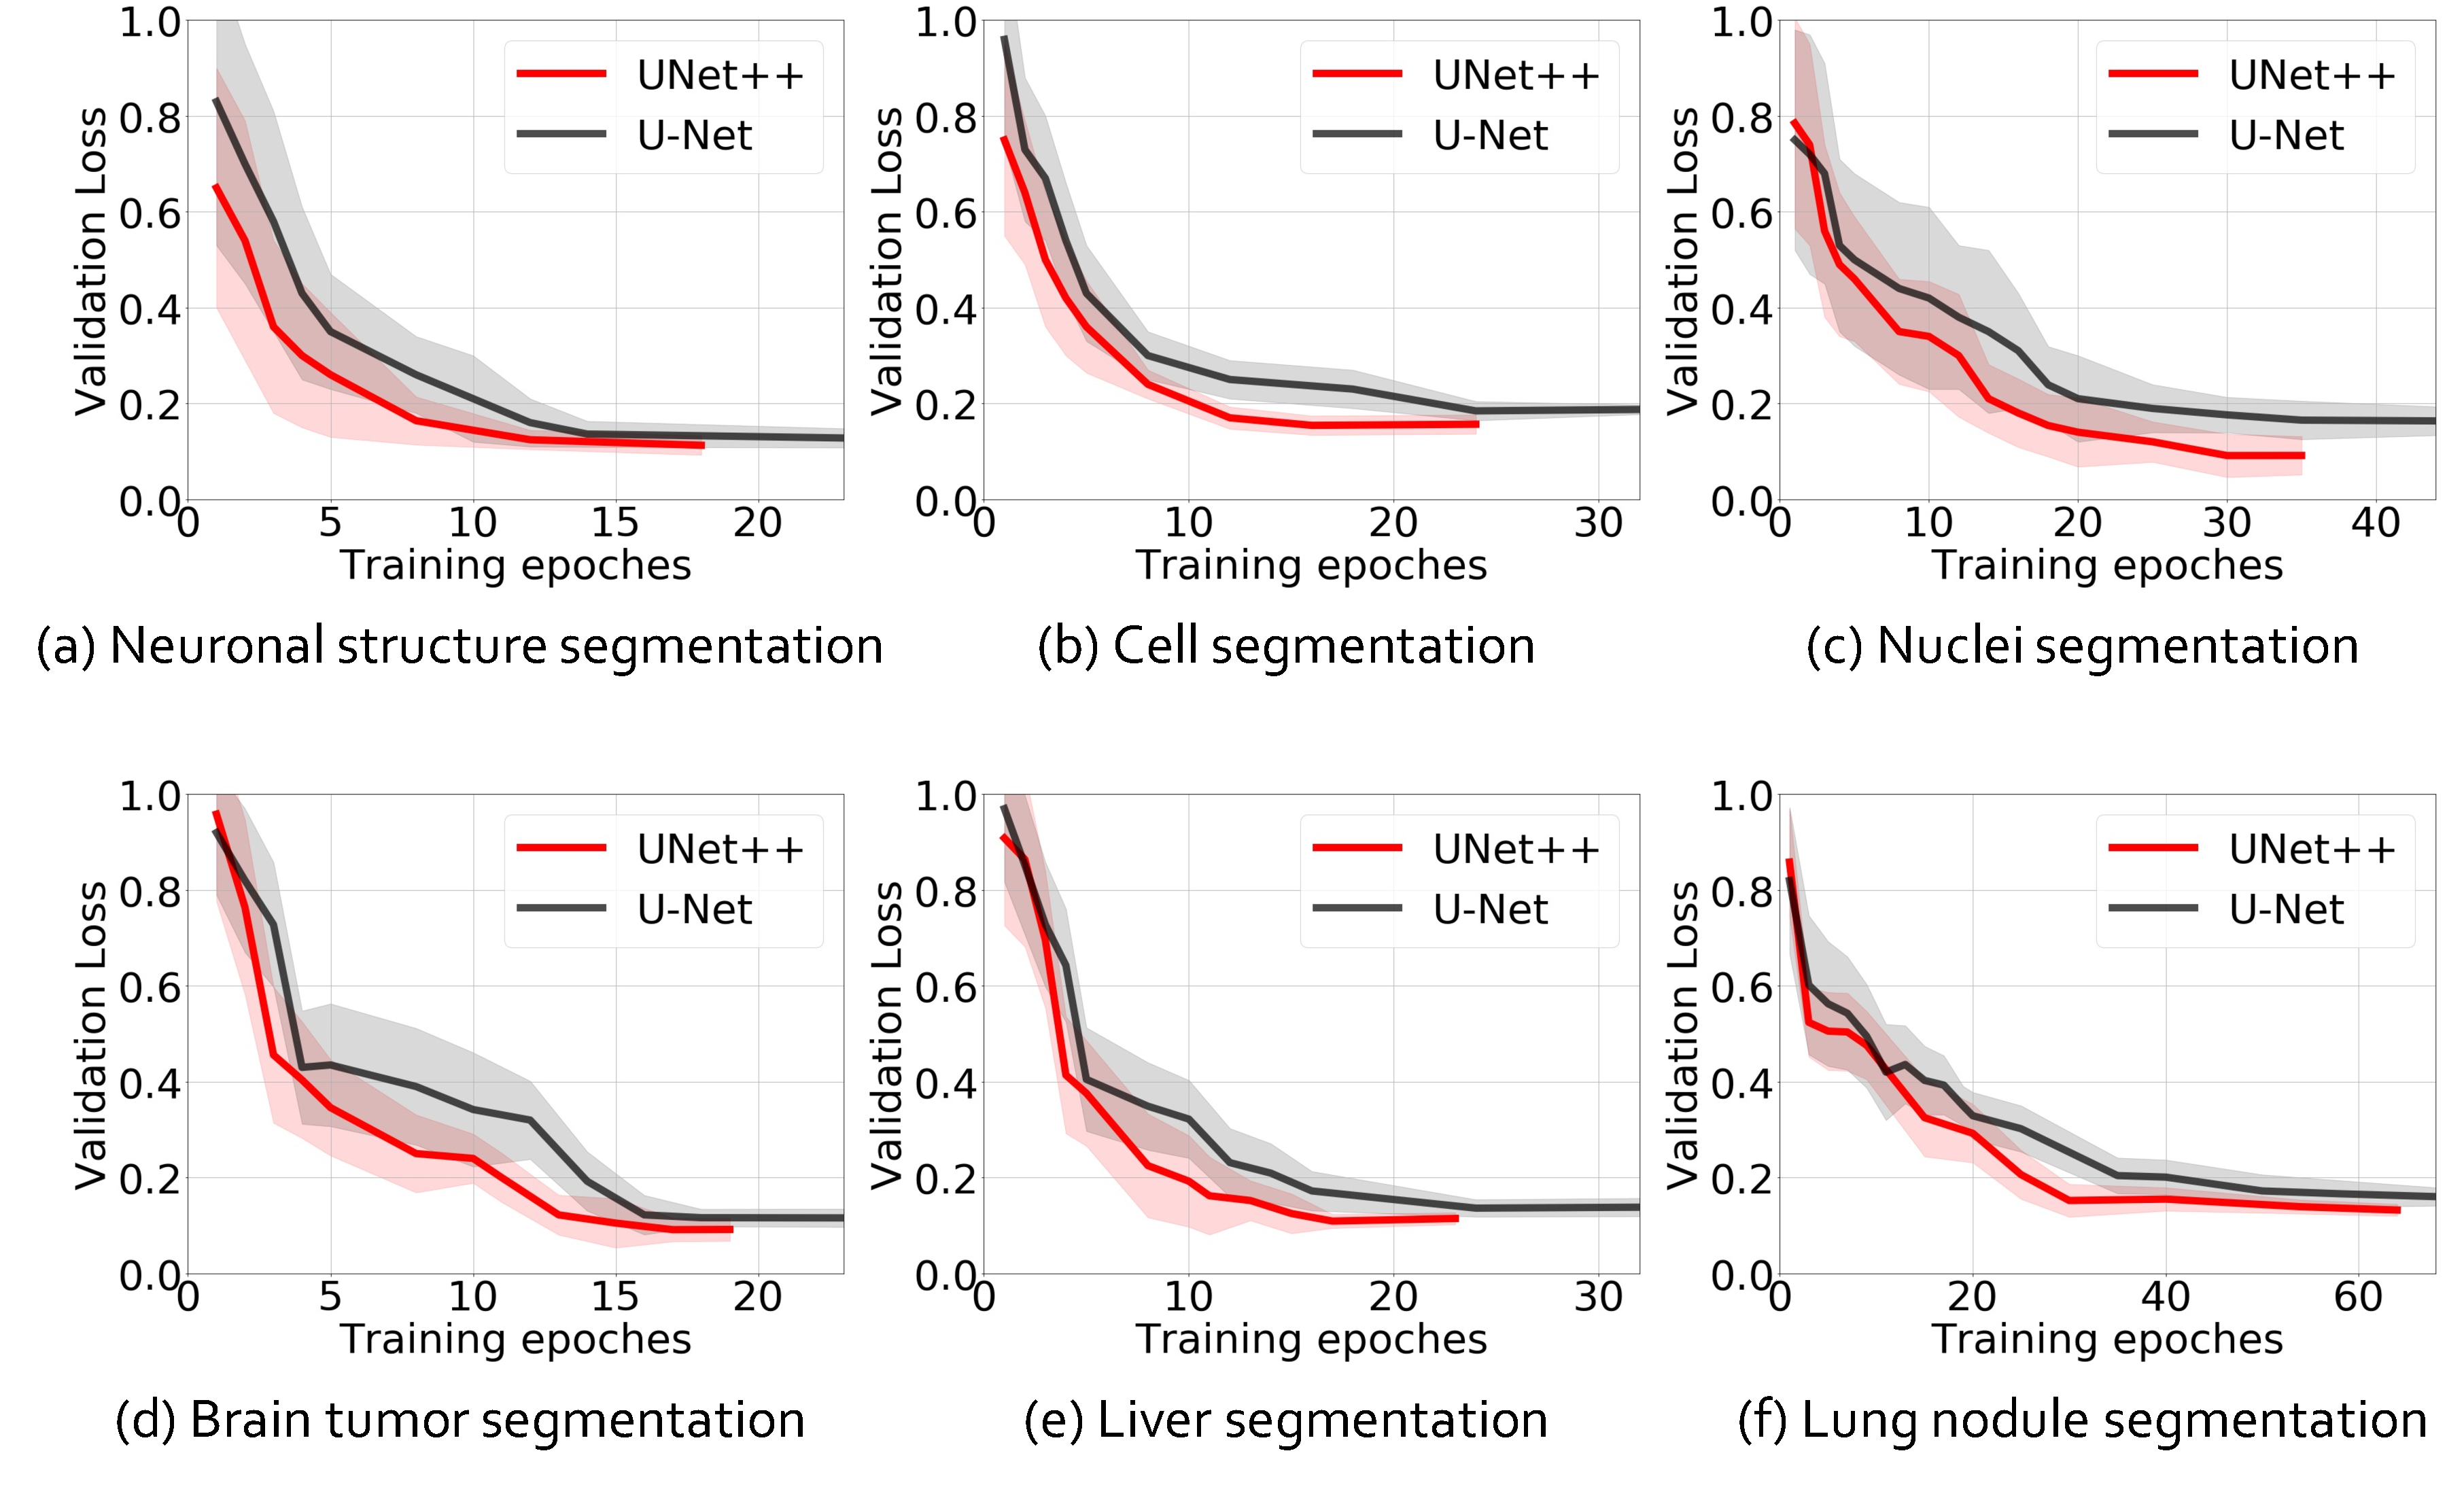
\includegraphics[width=1.0\linewidth]{Figures/CH4/fig_learning_curves.pdf}
\end{center}
\caption[UNet++ Enables a Better Optimization than U-Net]{
UNet++ enables a better optimization than U-Net evidenced by the learning curves for the tasks of neuronal structure, cell, nuclei, brain tumor, liver, and lung nodule segmentation. We have plotted the validation losses averaged by 20 trials for each application. As seen, UNet++ with deep supervision accelerates the convergence speed and yields the lower validation loss due to the new design of the intermediate layers and dense skip connections.}
\label{ch4:fig:learning_curves}
\end{figure}
%##############################################################################################



\subsection{How Do Multi-scale Feature Maps Aggregate in UNet++?}
\label{ch4:discussion_conclusion:feature_maps_visualization}

In Section~\ref{ch4:motiv}, we explained that the redesigned skip connections enable the fusion of semantically rich decoder feature maps with feature maps of varying semantic scales from the intermediate layers of the architecture. In this section, we illustrate this privilege of our re-designed skip connections by visualizing the intermediate feature maps.

\figurename~\ref{ch4:fig:feature_map_aggregation} shows representative feature maps from early, intermediate, and late layers along the top most skip connection (\ie X$^{0,i}$) for a brain tumor image. The representative feature map for a layer is obtained by averaging all its feature maps. Also note that architectures in the left side of \figurename~\ref{ch4:fig:feature_map_aggregation} are trained using only loss function appended to the deepest decoder layer (X$^{0,4}$) whereas the architectures in the right side of \figurename~\ref{ch4:fig:feature_map_aggregation} are trained with deep supervision. 
Note that these feature maps are not the final outputs. We have appended an additional 1$\times$1 convolutional layer on top of each decoder branch to form the final segmentation.
We observe that the outputs of U-Net's intermediate layers are semantically dissimilar  whereas for UNet+ and UNet++ the outputs are formed gradually. The output of node X$^{0,0}$ in U-Net undergoes slight transformation (few convolution operations only) whereas the output of X$^{1,3}$, the input of X$^{0,4}$, goes through nearly every transformation (four down-sampling and three up-sampling stages) learned by the network. Hence, there is a large gap between the representation capability of X$^{0,0}$ and X$^{1,3}$. So, simply concatenating the outputs of X$^{0,4}$ and X$^{1,3}$ is not an optimal solution. In contrast, redesigned skip connections in UNet+ and UNet++ help refine the segmentation result gradually. 
We further present the learning curves of all six medical applications in~\figurename~\ref{ch4:fig:learning_curves}, revealing that the addition of dense connections in UNet++ encourages a better optimization and reaches lower validation loss.


\subsection{Isolated Learning or Collaborative Learning?}
\label{ch4:discussion_conclusion:collarborative_learning}

Collaborative learning is known as training multiple classifier heads of the same network simultaneously on the same training data. It is found to improve the generalization power of deep neural networks~\citep{song2018collaborative}. UNet++ naturally embodies collaborative learning through aggregating multi-depth networks and supervising segmentation heads from each of the constituent networks. Besides, the segmentation heads, for example X$^{0,2}$ in \figurename~\ref{ch4:fig:prune_structure}, receive gradients from both strong (loss from ground truth) and soft (losses propagated from adjacent deeper nodes) supervision. As a result, the shallower networks improve their segmentation (\figurename~\ref{ch4:fig:pruned_vs_stand-alone}) and provide more informative representation to deeper counterparts. Basically, deeper and shallower networks regularize each other via collaborative learning in UNet++. Training multi-depth embedded networks together results in improved segmentation than training them individually as isolated network which is evident in \sectionname~\ref{ch4:embedded_vs_isolated_training}. The embedded design of UNet++ makes it amenable to auxiliary training, multi-task learning, and knowledge distillation~\citep{bengio2009learning,hinton2015distilling,song2018collaborative}.

% \subsection{Can UNet++ facilitate active learning in segmentation?}
% \label{ch4:discussion_conclusion:unetplusplus_active_learning_segmentation}


\subsection{Conclusion and Broader Impacts}
\label{ch4:discussion_conclusion:conclusion_broader_impacts}

We have presented a novel architecture, named UNet++, for more accurate image segmentation. The improved performance by our UNet++ is attributed to its nested structure and re-designed skip connections, which aim to address two key challenges of the U-Net: 1) unknown depth of the optimal architecture and 2) the unnecessarily restrictive design of skip connections. We have evaluated UNet++ using six distinct biomedical imaging applications and demonstrated consistent performance improvement over various state-of-the-art backbones for semantic segmentation and meta framework for instance segmentation.

We first presented UNet++ in our DLMIA 2018 paper~\citep{zhou2018unet++}. 
UNet++ has since been widely adopted by the research community, either as a strong baseline for comparison~\citep{sun2019high,fang2019selective,fang2019improved,meng2020multiscale}, or as a source of inspiration for developing newer semantic segmentation architectures~\citep{zhang2018mdu,chen2018improved,zhou2018learning,wu2019automatical,song2019u,yang2019eda}; it has also been utilized for multiple applications, not only for diseases/organs/tissues segmentation in biomedical images~\citep{zyuzin2019comparison,cui2019pulmonary}, but also for image coloring~\citep{di2021color}, moon impact crater detection~\citep{jia2021moon}, microseismic monitoring~\citep{guo2021first}. Recently, \citet{shenoy2019feature} has independently and systematically investigated UNet++ for the task of ``contact prediction model PconsC4'', demonstrating significant improvement over widely-used U-Net. 



% \section*{Acknowledgements}

% I thank Mohammad Reza Hosseinzadeh Taher and Fatemeh Haghighi for their verification of liver segmentation performance and the ablation study of embedded and isolated UNet++. I also thank Michael G. Meyer for allowing us to test our ideas on the Cell-CT dataset.